%%%%%%%%%%%%%%%%%%%%%%%%%%%%%%%%%%%%%%%%%%%%%%%%%%%%%%%%%%%%%%%%%%%%%%%%%%%%%%%%%%%%%%%%%%%%%%%%%%%
\documentclass[12pt, generalexam]{generalexam} % prospectus style
\usepackage[amssymb]{SIunits}                  % allows SI units
\usepackage[pdftex]{graphicx}                  % allows .eps and .epsi graphics to be inserted
\usepackage{epic}                              % allows use of latex graphics
\usepackage{eepic}                             % allows use of latex graphics
\usepackage{varioref}
\usepackage{amssymb,amsmath}                   % Amer. Math. Soc. packages
\usepackage{amsfonts}                          % Amer. Math. Soc. special fonts package
\usepackage[centerfoot]{pageno}                % allows positioning of page numbers
\usepackage{natbib} 		                   % citations with ametsoc.bst
\usepackage[table]{xcolor}                     % allow for alternating row colors in table
\bibpunct{(}{)}{;}{a}{}{,}                     % AMS refs are ``author year'' not ``author, year''
\usepackage{longtable}
\usepackage{array}
\usepackage{times}
\usepackage{hyperref}
\usepackage[bottom]{footmisc}
\usepackage{listings}
\labelformat{equation}{\textup{(#1)}}
\labelformat{enumi}{\textup{(#1)}}
% \usepackage{hyperref}
% \renewcommand{\sectionautorefname}{Section}
% \renewcommand{\chapterautorefname}{Chapter}
\makeatletter
\def\@seccntformat#1{\hb@xt@ 24px{\hfil\csname the#1\endcsname}\quad}
\makeatother
%%%%%%%%%%%%%%%%%%%%%%%%%%%%%%%%%%%%%%%%%%%%%%%%%%%%%%%%%%%%%%%%%%%%%%%%%%%%%%%%%%%%%%%%%%%%%%%%%%%
% control list spacing %
%%%%%%%%%%%%%%%%%%%%%%%%
\usepackage{setspace}
\let\olditemize=\itemize
\def\itemize{\olditemize\setlength{\itemsep}{-0.5ex}\setstretch{0.85}}
\renewcommand{\labelitemi}{$\star$}
%%%%%%%%%%%%%%%%%%%%%%%%%%%%%%%%%%%%%%%%%%%%%%%%%%%%%%%%%%%%%%%%%%%%%%%%%%%%%%%%%%%%%%%%%%%%%%%%%%%
% math shortcuts %
%%%%%%%%%%%%%%%%%%
\newcommand{\be}{\begin{equation}}                                  % begin equation environment
\newcommand{\ee}{\end{equation}}                                    % end equation environment
\newcommand{\bea}{\begin{eqnarray}}                                 % begin equation array environment
\newcommand{\eea}{\end{eqnarray}}                                   % end equation array environment
\newcommand{\dd}{\mathrm{d}}                                        % derivative d
\newcommand{\pd}[2]{\frac{\partial#1}{\partial#2}}                  % partial derivative
\newcommand{\pdd}[3]{\frac{\partial^{2}#1}{\partial#2 \partial#3}}  % second order partial derivative
\newcommand{\mbf}[1]{\mathbf{#1}}                                   % math bold font
\newcommand{\mc}[1]{\mathcal{#1}}                                   % math caligraphy font
\newcommand{\ol}[1]{\overline{#1}}                                  % math overline
\newcommand{\divider}{\vspace{7.5em}\hrule\vspace{1em}}               % big skip, line, small skip
%%%%%%%%%%%%%%%%%%%%%%%%%%%%%%%%%%%%%%%%%%%%%%%%%%%%%%%%%%%%%%%%%%%%%%%%%%%%%%%%%%%%%%%%%%%%%%%%%%%
% add revision information to footer %
%%%%%%%%%%%%%%%%%%%%%%%%%%%%%%%%%%%%%%
\IfFileExists{revision.sty}{\usepackage{revision}}{}
%%%%%%%%%%%%%%%%%%%%%%%%%%%%%%%%%%%%%%%%%%%%%%%%%%%%%%%%%%%%%%%%%%%%%%%%%%%%%%%%%%%%%%%%%%%%%%%%%%%
\newenvironment{blockquote}{\begin{quote}\itshape}{\end{quote}}
\lstnewenvironment{code}[1][]{\noindent\minipage{\linewidth}\vspace{0.5\baselineskip}\lstset{basicstyle=\ttfamily\footnotesize,frame=shadowbox,rulesepcolor=\color{black}, #1}}{\endminipage}
%%%%%%%%%%%%%%%%%%%%%%%%%%%%%%%%%%%%%%%%%%%%%%%%%%%%%%%%%%%%%%%%%%%%%%%%%%%%%%%%%%%%%%%%%%%%%%%%%%%
% table definitions
%%%%%%%%%%%%%%%%%%%
\newenvironment{telement}[2]{\begin{minipage}[c]{#1} \centering #2} {\end{minipage}}
\newcommand{\coremem}{\color{red}}
\newcommand{\member}[1]{\begin{telement}{0.66in}{#1}\end{telement}}
\newcommand{\ic}[1]{\begin{telement}{1in}{#1}\end{telement}}
\newcommand{\bc}[1]{\begin{telement}{1in}{#1}\end{telement}}
\newcommand{\radar}[1]{\begin{telement}{0.5in}{#1}\end{telement}}
\newcommand{\microphysics}[1]{\begin{telement}{1in}{#1}\end{telement}}
\newcommand{\lsm}[1]{\begin{telement}{0.66in}{#1}\end{telement}}
\newcommand{\pbl}[1]{\begin{telement}{0.66in}{#1}\end{telement}}
%%%%%%%%%%%%%%%%%%%%%%%%%%%%%%%%%%%%%%%%%%%%%%%%%%%%%%%%%%%%%%%%%%%%%%%%%%%%%%%%%%%%%%%%%%%%%%%%%%%


\begin{document}

\title{An Assessment of the Primary Scientific Challenges Facing\\the Warn-on-Forecast Initiative}
\author{PATRICK TIMOTHY MARSH}
\depositdate{2012}
\majorfield{SCHOOL OF METEOROLOGY}

%%%%%%%%%%%%%%%%%%%%%%%%%%%%%%%%%%%%%%%%%%%%%%%%%%%%%%%%%%%%%%%%%%%%%%%%%%%%%%%%%%%%%%%%%%%%%%%%%%%
\begin{preface}
% space avoids a problem, keep it

\tableofcontents
% \listoftables
\listoffigures

\doublespacing
\prefacesection{Statement of Problem}
\label{sproblem}
%!TEX root = generalexam.tex


% BEGIN STATEMENT OF PROBLEM

The convective-scale ``Warn-on-Forecast'' paradigm (WoF) includes explicit numerical prediction of hazardous weather elements such as tornadoes, downbursts, and large hail. Current operational numerical modeling systems are not designed for the time and space scales on which these phenomena typically occur. Furthermore, the inherent predictability of these phenomena is not firmly established. These limitations alone present significant challenges for the WoF initiative. For the written portion of your general examination, provide an assessment of the primary scientific challenges facing the WoF effort, including a detailed summary of the theoretical and practical obstacles in these specific components of the WoF program:

    \bigskip\medskip
    \begin{enumerate}
        \item Assimilation of radar data (radial velocity and reflectivity), including the basis for and strengths/weaknesses of 3DVAR, 4DVAR, EnKF, and others, including hybrid approaches;
        \item Error growth and predictability on the convective scale; and
        \item Development, testing, optimization, and application of convective-scale ensembles
    \end{enumerate}
    \medskip

For this task, information is to be gathered from books, journals, and online resources, but not from personal communication with scientists currently working on the WoF project. All sources of information are to be documented as they would be for the scientific literature. If you need further clarification on this assignment, please contact your Committee Co-Chair. Your written summary will be due one month from the date you receive this letter. Please submit the summary to the entire committee as a PDF file.





% \prefacesection{Executive Summary}
% \label{esummary}
% %!TEX root = generalexam.tex


% BEGIN EXECUTIVE SUMMARY

The Warn-on-Forecast (WoF) initiative is tasked with establishing the scientific acumen to transform the severe convective weather warning paradigm from one based on detection to one based on prediction. The underlying idea behind WoF is to create the capability to issue warnings for severe convective hazards based on reliable, high-resolution numerical forecast guidance, instead of waiting until a severe convective hazard is observed, detected, or thought to be imminent \citep{stensrud2009wof}. Significant scientific questions must be answered and significant hurdles must be overcome before this vision can be achieved. Some of these hurdles are practical; some are theoretical; and some are even financial.


Data assimilation continues to be a source of active research for the WoF initiative. Advancements have been made from utilizing hand analyses for initializing numerical models to choosing between variational analyses methods and enesemle kalman methods.

Achieving the WoF vision is hard. Very hard. It will require significant investments of intellection capital on many fronts.





\prefacesection{Acknowledgements}
\label{acknowledgements}
%!TEX root = generalexam.tex

% BEGIN ACKNOWLEDGEMENTS

This document was prepared in the span of 30 days in accordance to the rules put forth by the School of Meteorology's requirements for the General Examination. This work should be considered the thoughts and opinions of the author, and do not represent the opinions of his advisors.


Additionally, the author had very little knowledge of data assimilation when the project began. The first half of the allotted time was devoted to learning as much as possible about data assimilation. Everything from this time frame was, and still is, a blur. When it came time to write the report, it was very difficult to remember what source of information resulting in what knowledge. Thus, the author would like to acknowledge the following references that contributed to his understanding of data assimilation. This task would not have been able to be completed --- at least not with whatever sanity he has left --- without their willingness to make their papers, presentations, and lecture notes available online to the greater scientific community. In no particular order:

\vspace{2em}
\begin{itemize}
    \item \cite{evensen1994enkf} and \cite{evensen2003enkf}
    \vspace{1em}
    \item The ECMWF Lecture Series [Available online at: \url{http://www.ecmwf.int/newsevents/training/rcourse_notes}
    \vspace{1em}
    \item The power point presentations of Dr. Dale Barker from the Korean Meteorological Administration's Data Assimilation Workshops. Presentations can be found online at \url{http://weather.snu.ac.kr}
    \vspace{1em}
    \item A Presentation on Data Assimilation by Ms. Sarah L. Dance. [Available online at: \url{http://www.icfd.rdg.ac.uk/Workshops/Mathematics%20and%20Applications%20of%20Data%20Assimilation/S_Dance.pdf}]
    \vspace{1em}
\end{itemize}


\noindent Additionally, the author promised to convey that this document was written without the aid of caffeinated beverages (such as coffee, soda, or energy drinks). This document was written with the aid of lots of decaf iced-tea, many dozen homemade Reeses Pieces Peanut Butter cookies backed by his wife, and the sheer desire to complete his PhD.
\end{preface}
%%%%%%%%%%%%%%%%%%%%%%%%%%%%%%%%%%%%%%%%%%%%%%%%%%%%%%%%%%%%%%%%%%%%%%%%%%%%%%%%%%%%%%%%%%%%%%%%%%%

\doublespacing

% INTRODUCTION
\chapter{Introduction}
\label{introduction}
%!TEX root = generalexam.tex


% BEGIN CHAPTER

The Warn-on-Forecast (WoF) initiative is tasked with establishing the scientific acumen to transform the severe convective weather warning paradigm from one based primarily on detection to one based more on prediction. The underlying idea behind WoF is to create the capability to issue warnings for severe convective hazards based on reliable, high-resolution numerical forecast guidance, instead of waiting until a severe convective hazard is observed, detected, or thought to be imminent \citep{stensrud2009wof}. However, significant hurdles must be overcome for this vision to become a reality.


The prospect of fundamentally shifting the prevailing paradigm in the convective-scale numerical modeling community, such as WoF proposes doing, is not without precedent. In 1990, Douglas Lilly challenged the status quo by rhetorically asking if the time had come for cloud-resolving scale forecasts of a predictive ability \citep{lilly1990}. Lilly recognized this would not be easy. He discussed numerous scientific hurdles, but stressed that through collaboration across agencies; renewed emphasis on predictability studies; and improvements in observations, data assimilation and model parameterizations, the challenge was surmountable in the coming decade --- and he was right! Operational, semi-operational, and research centers now regularly produce contiguous United States (CONUS) or near-CONUS scale numerical forecasts with grid spacing \mbox{O(1 km)} without the use of convective parameterization schemes. More importantly, these forecasts produce useful guidance of convective initiation (preliminary results from the 2011 HWT Experimental Forecast Program), reasonably accurate depictions of convective evolution (e.g., \citealp{clark2012overview, clark2010mcv, clark2010verification, clark2009comparison, schwartz2009camresolution, kain2010attributes, kain2008camconsiderations, done2004cams}), and improved forecasts of precipitation \citep{novak2011qpf}.


Fast forward 20 years and the convective hazards research community is once again being pushed to alter how it approaches the prediction of high-impact convective hazards -- this time through the WoF initiative. Many of the challenges laid forth by \cite{lilly1990} will once again have to be reexamined. Although the realm of data assimilation has experienced rapid advancements, determining the initial states of numerical models remains a significant challenge; studies on predictability and error growth will help to frame the WoF vision by placing bounds on reasonable expectations; and discussions on convective-scale ensembles will frame how WoF is implemented and the resources needed for it to achieve fruition. The WoF initiative will require close collaboration across research organizations; it will push the bounds of computational resources; and will require the development of new approaches to tackle old problems -- especially the need for efficient numerical techniques involved in data assimilation.









% RADAR DATA ASSIMILATION
\chapter{Assimilation of Radar Data}
\label{data_assimilation}
%!TEX root = generalexam.tex

% BEGIN CHAPTER

%%%%%%%%%%%%%%%%%%%%%%%%%%%%%%%%%%%%%%%%%%%%%%
\section{The origins of Data Assimilation}
\label{The origins of Data Assimilation}
%%%%%%%%%%%%%%%%%%%%%%%%%%%%%%%%%%%%%%%%%%%%%%

As early as the mid-1800s, hand-analyses of weather observations were being drawn to gain insights into various atmospheric phenomena. For example, \cite{redfield1841observations} produced hand analyses of a strong cold-season extratropical cyclone over the warm-waters of the Gulf Stream Current located just south of Cape Cod, Massachusetts (what is now referred to as a Nor'Easter) in an effort gain scientific insight. Hand analyses were the only method of generating a representation of the true state of the atmosphere until the invention of the computer, when numerical analyses became possible. The first such attempt at an objective analysis done via computers was done by \cite{panofsky1949oban}, when he used third-degree polynomials fit to observations over a relatively limited area to represent the distribution of meteorological variables.


A few years later, \cite{gilchrist1954oban} extended the work of \cite{panofsky1949oban} by creating objective analyses that utilized polynomial expansion, but only for observations within a radius of influence around each observation. They went on to compare numerical forecasts initialized from subjective analyses to those initialized with this new objective analysis approach and found that numerical forecasts initialized with the objective analyses verified better than the forecasts initialized with the subjective analyses. Gilchrist and Cressman attributed these results to the fact that objective analyses, using their method, forced geostrophic balance on the analyses which, in turn, produced analyses that fared better in a quasi-geostrophic model. This finding would ultimately have a profound impact on how to perform objective analysis and data assimilation for use in generating initial conditions in numerical models.


\cite{gilchrist1954oban} also introduced the notion of using a previous numerical forecast as an estimate of the analysis, or background field. This was built upon by \cite{bergthorsson1955numerical} who framed the analysis problem in terms of making incremental changes to a background field. This approach utilized a statistically weighted linear combination of nearby observations and the background field. This process could then be repeated to further refine the analysis, although the first pass typically produced satisfactory results. \cite{bergthorsson1955numerical} recognized that it was most likely hopeless to try and obtain a ``\emph{true} analysis of the atmosphere'', but rather the role of objective analysis is to produce the ``\emph{most probable} analysis''. A variation on the iterative technique proposed by \cite{bergthorsson1955numerical} was implemented as the operational objective analysis system at the Joint Numerical Weather Prediction Unit in the late 1950s \citep{cressman1959operational}.


In 1954, \cite{eliassen1954oi} proposed a statistical-based objective analysis technique, often called \emph{optimal interpolation}, or more aptly \emph{statistical interpolation}. At the same time Eliassen was developing statistical interpolation, Sasaki was developing a deterministic-based objective analysis technique employing the variational principle from calculus of variations (e.g., \citealp{sasaki1955variational, sasaki1958objective, sasaki19694dvariational, sasaki1970variational, sasaki1970numerical, sasaki1970weakconstraint}, etc.). This technique ultimately laid the foundation for the 3D-Variational (3DVAR) and 4D-Variational (4DVAR) data assimilation schemes.



%%%%%%%%%%%%%%%%%%%%%%%%%%%%%%%%%%%%%%%%%%%%%%%%%%%%%%%%%%%
\section{The Mathematics of Analysis and Data Assimilation}
\label{The Mathematics of Analysis and Data Assimilation}
%%%%%%%%%%%%%%%%%%%%%%%%%%%%%%%%%%%%%%%%%%%%%%%%%%%%%%%%%%%

The tenets of a good analysis are fairly straight forward. One variation on these tenets is given:


    \begin{enumerate}
        \item Begin with a good quality first guess, or background, (i.e., a previous analysis or forecast).
        \item The analysis should be closest to the data most trusted. Conversely, areas of suspicious data should be given little weight.
        \item When observations are dense assume the true state is near the average of the observations.
        \item The analysis should be smooth, honoring known relationships and balances.
        \item The analysis should respect known features of the system.
    \end{enumerate}


\noindent To put this another way, the background state and observations are important sources of information in an analysis, but neither can be completely trusted. This is because sources of errors exist in both the observations (e.g., instrument errors) and in the model that produced the background field (e.g., inadequate model physics or grid spacing). A good analysis scheme seeks to minimize the average difference between the analysis and the true atmospheric state\footnote{When creating an analysis for numerical weather prediction, the additional constraint of producing an analysis that adheres to the model's required balances is added, as identified by \cite{gilchrist1954oban}.}. Thus, the creation of a good analysis is an exercise in optimization theory. Typically the analysis that produces the smallest mean squared error when compared to the true atmospheric state is called the \emph{\textbf{best}} analysis.


A popular adage in computer programming is ``Garbage in, Garbage out''. In the context of numerical weather prediction this translates to ``Poor Initial Analysis, Poor Forecast''. Even before the advent of computers, \cite{bjerknes1904nwpvision} postulated that in order to produce numerical forecasts of subsequent states of the atmosphere that:


\begin{blockquote}
    \begin{enumerate}
        \item One has to know with sufficient accuracy the state of the atmosphere at a given time; and
        \item One has to know with sufficient accuracy the laws according to which one state of the atmosphere develops from another.
    \end{enumerate}
\end{blockquote}


\noindent Bjerknes recognized that the creation of sufficiently accurate analysis of the atmosphere is a necessary condition for reliable forecasts of future atmospheric states based on the integration of the governing equations.


In the context of creating the best analysis for use in numerical weather prediction, the choice of forecast model is critical and must be made first. The model choice has a direct impact on the creation of the analysis, as it establishes the discrete basis on which the analysis will occur. After choosing the model, the entire state of the atmosphere at a single time needs to be represented in model space. This background state can be in the form of grid points, spherical harmonic coefficients, etc, and contains atmospheric variables (e.g., temperatures, wind components, etc.) and is denoted by vector $\mbf{x}_b$. Similarly the observations of the atmosphere can be represented by vector $\mbf{y}$, which consists of observations of different fields at different locations, not necessarily the same locations as $\mbf{x_b}$.


Since no requirement is made that observations are collocated with model space, there is no guarantee that a surjection, or one-to-one mapping, exists between $\mbf{y}$ and $\mbf{x_b}$. Thus, it is assumed that the model is always possible to determine ``model equivalents'' of observations. Mathematically speaking this implies that an \emph{\textbf{observation operator}}, or\emph{\textbf{forward operator}}, $\mc{H}$, exists such that


    \be
        \label{observation operator}
        \mbf{y} = \mc{H}(\mbf{x})
    \ee


\noindent where $\mbf{x}$ is any model-space vector. Simply stated, the observation operator takes model-space vectors and remaps them such that they can be directory compared to observation-space vectors.\footnote{One way of thinking about the resulting vector is that it consists of the model equivalents previously mentioned.} The assumption is made that $\mc{H}$ does not introduce any errors, implying that


    \be
        \label{perfect observation operator}
        \mbf{y^*} = \mc{H}(\mbf{x^*})
    \ee


\noindent where $\mbf{x^*}$ is the true state of the atmosphere depicted in model-space and $\mbf{y^*}$ are the true values of all observations (i.e., there are no instrument errors contained in the observations). In the general case, it is required that error-free inputs ($\mbf{x_b} = \mbf{x^*}$ and $\mbf{y} = \mbf{y^*}$) into $\mc{H}$ produces an error-free analysis ($\mbf{x_a}=\mbf{x^*}$). Thus, it is assumed, at least at this point of the derivation, that the observation operator is a perfect operator and does not introduce error into an analysis. It will be shown later that this is certainly not always the case.


The process by which one guarantees the best analysis, for a given observation operator, is known as Kalman filtering, with a basis in linear least squares analysis.  Kalman filtering methods have been derived under two general frameworks: \emph{\textbf{minimum variance}} and \emph{\textbf{maximum likelihood}}. Derivations of the Kalman filtering equations in each of these frameworks follow.




%%%%%%%%%%%%%%%%%%%%%%%%%%%%%%%%%%%%%%%%%%%
\subsection{The Minimum Variance Framework}
\label{The Minimum Variance Framework}
%%%%%%%%%%%%%%%%%%%%%%%%%%%%%%%%%%%%%%%%%%%

Data assimilation is designed to ``perfectly'' blend information collected from numerous observations through the use of past analyses and model and physical constraints. Therefore, starting from the results of \cite{bergthorsson1955numerical}, data assimilation can be denoted mathematically as a simple linear combination of the background field, the model equivalents, the observations, and a vector of constants.


\be
    \label{multivariate linear combination}
    \mbf{x_a} = \mbf{Fx_b} + \mbf{G}\mc{H}(\mbf{x_b}) + \mbf{Ky} + \mbf{c}
\ee


\noindent where $\mbf{x_a}$ is the model analysis, $\mbf{F}$, $\mbf{G}$, and $\mbf{K}$ are matrices and $\mbf{c}$ is a vector of constants.


Recalling that error-free inputs are assumed to result in an error free analysis, \ref{multivariate linear combination} can be rewritten as:


\be
    \label{error-free analysis-1}
    \mbf{x^*} = \mbf{Fx^*} + \mbf{G}\mc{H}(\mbf{x^*}) + \mbf{Ky^*} + \mbf{c}.
\ee


\noindent Using \ref{perfect observation operator}, and exploiting the multiplicative identity of matrices, $\mbf{x} = \mbf{Ix}$, \ref{error-free analysis-1} can be rewritten as


\be
    \label{error-free analysis-2}
    \mbf{Ix^*} = \mbf{Fx^*} + \mbf{G}\mc{H}(\mbf{x^*}) + \mbf{K}\mc{H}(\mbf{x^*}) + \mbf{c}.
\ee


\noindent However, since \ref{error-free analysis-2} holds for all values $\mbf{x^*}$, $\mbf{c}$ must be $\mbf{0}$, and \ref{error-free analysis-2} can generalized to,


\be
    \label{error-free analysis-3}
    \mbf{I} = \mbf{F} + \mbf{G}\mc{H}(\cdot) + \mbf{K}\mc{H}(\cdot).
\ee


\noindent Rearranging terms, it is shown that


\be
    \label{reduction of terms}
    \mbf{F} + \mbf{G}\mc{H}(\cdot) = \mbf{I} - \mbf{K}\mc{H}(\cdot).
\ee


\noindent Plugging \ref{reduction of terms}, into \ref{multivariate linear combination}, and recalling that $\mbf{c} = \mbf{0}$, the dependencies on $\mbf{F}$, $\mbf{G}$, and $\mbf{c}$ are removed:


\be
    \label{expanded analysis equation}
    \mbf{x_a} = \mbf{x_b} - \mbf{K}\mc{H}(\mbf{x_b}) + \mbf{Ky}.
\ee


\be
    \label{full analysis equation}
    \mbf{x_a} = \mbf{x_b} + \mbf{K}(\mbf{y} - \mc{H}(\mbf{x_b})).
\ee


\ref{full analysis equation} is the general form of the multidimensional analysis equation and $\mbf{K}$ is called the \emph{\textbf{gain matrix}}. The gain matrix is used to transform information defined in observation-space to model-space, by essentially assigning weights to each observational piece of information. Unfortunately, \ref{full analysis equation} does not guarantee to give the best analysis -- merely \emph{an} analysis. The Gauss-Markov theorem states, however, that in a linear regression the best linear unbiased estimator of the coefficients is given by the ordinary least squares estimator. This theorem assumes that the expected value of errors is zero and the errors are uncorrelated and have equal variances. Therefore, the best analysis is guaranteed when the gain matrix is chosen such that it minimizes the variance of the analysis error, under the assumptions denoted.


To determine this optimal gain matrix, the errors associated with the analysis, background, and observations are needed. These can be defined as


\be
    \label{analysis error}
    \epsilon_a = \mbf{x_a} - \mbf{x^*}
\ee


\be
    \label{background error}
    \epsilon_b = \mbf{x_b} - \mbf{x^*}
\ee


\be
    \label{observation error}
    \epsilon_o = \mbf{y} - \mbf{y^*}
\ee


\noindent where \ref{analysis error} defines the analysis error as the difference between the model produced analysis and the true state of the atmosphere in model-space, \ref{background error} defines the background error as the difference between the background field and the true state of the atmosphere depicted in model space, and \ref{observation error} defines the observation error as the difference between the observation vector and the state of the atmosphere. It is also assumed that the errors are sufficiently small such that


\be
    \label{linearized observation operator}
    \mc{H}(\mbf{x_b}) = \mc{H}(\mbf{x^*}) + \mbf{H}\epsilon_b + \text{O}(\epsilon_b^2)
\ee


\noindent where $\mbf{H}$ is the Jacobian of $\mc{H}$, and O$(\epsilon_b^2) \approx 0$. This assumption is known as the \emph{\textbf{tangent linear hypothesis}}. Substituting \ref{linearized observation operator}, the expressions for the error fields, and \ref{perfect observation operator} into the analysis equation given in \ref{full analysis equation}, an expression for the analysis error can be derived:


$$
    \epsilon_a + \mbf{x^*} = \epsilon_b + \mbf{x^*} + \mbf{K}\left[\epsilon_o + \mbf{y^*} - \mc{H}(\mbf{x^*}) - \mbf{H}\epsilon_b \right],
$$


$$
    \epsilon_a = \epsilon_b + \mbf{K}\left[\epsilon_o + \mbf{y^*} - \mbf{y^*} - \mbf{H}\epsilon_b \right],
$$


$$
    \epsilon_a = \epsilon_b + \mbf{K}\left[\epsilon_o - \mbf{H}\epsilon_b \right],
$$


$$
    \epsilon_a = \epsilon_b + \mbf{K}\epsilon_o - \mbf{K}\mbf{H}\epsilon_b,
$$


$$
    \epsilon_a = \epsilon_b - \mbf{K}\mbf{H}\epsilon_b + \mbf{K}\epsilon_o,
$$


\be
    \label{expanded analysis error}
    \epsilon_a = \left(I - \mbf{K}\mbf{H}\right)\epsilon_b + \mbf{K}\epsilon_o.
\ee


As previously written, in order to satisfy the Gauss-Markov Theorem, the variance of the resulting analysis needs to be a minimum. Fortunately, the variances are contained in a larger matrix called the covariance matrix. Covariance matrices can be found by taking the expected value of each element of an outer product between a vector and itself. Mathematically this is represented by


$$
    \ol{\mbf{x}\mbf{x}^T}.
$$


\noindent The covariance matrix of the analysis error can then be given by:


$$
    \ol{\epsilon_a\epsilon_a^T} = \ol{\left[\left(\mbf{I}-\mbf{KH}\right)\epsilon_b+\mbf{K}\epsilon_o\right]\left[\left(\mbf{I}-\mbf{KH}\right)\epsilon_b+\mbf{K}\epsilon_o\right]^T},
$$


$$
    \ol{\epsilon_a\epsilon_a^T} = \ol{\left[\left(\mbf{I}-\mbf{KH}\right)\epsilon_b+\mbf{K}\epsilon_o\right] \left[\left(\left(\mbf{I}-\mbf{KH}\right)\epsilon_b\right)^T+\left(\mbf{K}\epsilon_o\right)^T\right]},
$$


$$
    \ol{\epsilon_a\epsilon_a^T} = \ol{\left[\left(\mbf{I}-\mbf{KH}\right)\epsilon_b+\mbf{K}\epsilon_o\right] \left[\left(\epsilon_b^T-\epsilon_b^T\mbf{H}^T\mbf{K}^T\right)+\epsilon_o^T\mbf{K}^T\right]},
$$


\bea \nonumber
    \label{expanded analysis error covariance}
    \ol{\epsilon_a\epsilon_a^T} &=&
    \ol{\left(\mbf{I}-\mbf{KH}\right)\epsilon_b\epsilon_b^T\left(\mbf{I}-\mbf{KH}\right)^T} + \\ &&
    \ol{\left(\mbf{I}-\mbf{KH}\right)\epsilon_b\epsilon_o^T\mbf{K}^T +
    \mbf{K}\epsilon_o\epsilon_b^T(\mbf{I}-\mbf{KH})^T + \mbf{K}\epsilon_o\epsilon_o^T\mbf{K}^T}.
\eea


\noindent Making the assumption that the background and observation errors are uncorrelated (i.e., $\ol{\epsilon_b\epsilon_o^T} = 0 = \ol{\epsilon_o\epsilon_b^T}$), \ref{expanded analysis error covariance} becomes


\be
    \label{analysis error covariance expanded}
    \ol{\epsilon_a\epsilon_a^T} =
    \left(\mbf{I}-\mbf{KH}\right)\ol{\epsilon_b\epsilon_b^T}\left(\mbf{I}-\mbf{KH}\right)^T + \mbf{K}\ol{\epsilon_o\epsilon_o^T}\mbf{K}^T.
\ee


\noindent To save space, the error covariances will be denoted by:


$$
    \mbf{P_a} \equiv \ol{\epsilon_a\epsilon_a^T},
$$


$$
    \mbf{B} \equiv \ol{\epsilon_b\epsilon_b^T},
$$


$$
    \mbf{R} \equiv \ol{\epsilon_o\epsilon_o^T},
$$


\noindent and \ref{analysis error covariance expanded} can be rewritten as:


\be
    \label{analysis error covariance}
    \mbf{P_a} =
    \left(\mbf{I}-\mbf{KH}\right)\mbf{B}\left(\mbf{I}-\mbf{KH}\right)^T +
    \mbf{K}\mbf{R}\mbf{K}^T.
\ee


In a covariance matrix, the variances are conveniently located along its diagonal. Thus, minimizing the analysis error variance is equivalent to minimizing the sum of the diagonal elements, or trace, of the analysis error covariance matrix, and solving for $\mbf{K}$. Mathematically, this is given by


$$
    \pd{trace(\mbf{P}_a)}{\mbf{K}} = 0,
$$


$$
    \pd{trace(\mbf{P}_a)}{\mbf{K}} = \pd{}{\mbf{K}}\left[\left(\mbf{I}-\mbf{KH}\right)\mbf{B}\left(\mbf{I}-\mbf{KH}\right)^T + \mbf{KRK}^T\right]= 0,
$$


$$
    \pd{}{\mbf{K}}\left[\left(\mbf{B}-\mbf{KHB}\right)\left(\mbf{I}-\mbf{H}^T\mbf{K}^T\right)\right] + \pd{}{\mbf{K}}\left[\mbf{KRK}^T\right]= 0,
$$


$$
    \pd{}{\mbf{K}}\left[\mbf{B} - \mbf{BH}^T\mbf{K}^T - \mbf{KHB} + \mbf{KHBH}^T\mbf{K}\right] + \mbf{K}\left(\mbf{R} + \mbf{R}^T\right)= 0,
$$


$$
    \pd{}{\mbf{K}}\left[\mbf{B}\right] - \pd{}{\mbf{K}}\left[\mbf{BH}^T\mbf{K}^T\right] - \pd{}{\mbf{K}}\left[\mbf{KHB}\right] + \pd{}{\mbf{K}}\left[\mbf{KHBH}^T\mbf{K}\right] + \mbf{K}\left(\mbf{R} + \mbf{R}^T\right)= 0,
$$


$$
    0 - \mbf{BH}^T - [\mbf{HB}]^T + \mbf{K}[\mbf{HBH}^T + (\mbf{HBH}^T)^T] + \mbf{K}\left(\mbf{R} + \mbf{R}^T\right)= 0,
$$


$$
    -\mbf{BH}^T - \mbf{B}^T\mbf{H}^T + \mbf{K}[\mbf{HBH}^T + \mbf{HB}^T\mbf{H}^T] + \mbf{K}\left(\mbf{R} + \mbf{R}^T\right)= 0.
$$


\noindent This can be simplified further by noting that the error covariance matrices are symmetric and therefore equal to their transpose.


$$
    -\mbf{BH}^T - \mbf{BH}^T + \mbf{K}[\mbf{HBH}^T + \mbf{HBH}^T] + \mbf{K}\left(\mbf{R} + \mbf{R}\right)=0,
$$


$$
    -2\mbf{BH}^T + 2\mbf{KHBH}^T + 2\mbf{KR} = 0,
$$


$$
    -\mbf{BH}^T + \mbf{KHBH}^T + \mbf{KR} = 0,
$$


$$
    \mbf{KHBH}^T + \mbf{KR} = \mbf{BH}^T,
$$


$$
    \mbf{K}[\mbf{HBH}^T + \mbf{R}] = \mbf{BH}^T,
$$


\be
    \label{kalman gain matrix}
    \mbf{K} = \mbf{BH}^T[\mbf{HBH}^T + \mbf{R}]^{-1},
\ee


\noindent where the $\mbf{K}$ given by \ref{kalman gain matrix} is called the \emph{\textbf{Kalman Gain Matrix}}. The Gauss-Markov Theorem guarantees that the Kalman Gain Matrix provides the `best' analysis for a given $\mc{H}$.


Alternatively, the Kalman Gain Matrix can be, and often is, represented as


$$
    \mbf{K} = \mbf{BH}^T[\mbf{HBH}^T + \mbf{R}]^{-1},
$$


$$
    [(\mbf{B})^{-1} + \mbf{H}^T\mbf{R}^{-1}\mbf{H}]\mbf{K} = [(\mbf{B})^{-1}\mbf{H}^T\mbf{R}^{-1}\mbf{H}]\mbf{BH}^T[\mbf{HBH}^T + \mbf{R}]^{-1},
$$


$$
    [(\mbf{B})^{-1} + \mbf{H}^T\mbf{R}^{-1}\mbf{H}]\mbf{K} = [(\mbf{B})^{-1}\mbf{BH}^T + \mbf{H}^T\mbf{R}^{-1}\mbf{H}\mbf{BH}^T][\mbf{HBH}^T + \mbf{R}]^{-1},
$$


$$
    [(\mbf{B})^{-1} + \mbf{H}^T\mbf{R}^{-1}\mbf{H}]\mbf{K} = [\mbf{H}^T + \mbf{H}^T\mbf{R}^{-1}\mbf{H}\mbf{BH}^T][\mbf{HBH}^T + \mbf{R}]^{-1},
$$


$$
    [(\mbf{B})^{-1} + \mbf{H}^T\mbf{R}^{-1}\mbf{H}]\mbf{K} = \mbf{H}^T[\mbf{I} + \mbf{R}^{-1}\mbf{H}\mbf{BH}^T][\mbf{HBH}^T + \mbf{R}]^{-1},
$$


$$
    [(\mbf{B})^{-1} + \mbf{H}^T\mbf{R}^{-1}\mbf{H}]\mbf{K} = \mbf{H}^T\mbf{R}^{-1}[\mbf{R} + \mbf{H}\mbf{BH}^T][\mbf{HBH}^T + \mbf{R}]^{-1},
$$


$$
    [(\mbf{B})^{-1} + \mbf{H}^T\mbf{R}^{-1}\mbf{H}]\mbf{K} = \mbf{H}^T\mbf{R}^{-1}[\mbf{H}\mbf{BH}^T + \mbf{R}][\mbf{HBH}^T + \mbf{R}]^{-1},
$$


$$
    [(\mbf{B})^{-1} + \mbf{H}^T\mbf{R}^{-1}\mbf{H}]\mbf{K} = \mbf{H}^T\mbf{R}^{-1}\mbf{I},
$$


$$
    [(\mbf{B})^{-1} + \mbf{H}^T\mbf{R}^{-1}\mbf{H}]\mbf{K} = \mbf{H}^T\mbf{R}^{-1},
$$


\be
    \label{alternative kalman gain matrix}
    \mbf{K} = [(\mbf{B})^{-1} + \mbf{H}^T\mbf{R}^{-1}\mbf{H}]^{-1}\mbf{H}^T\mbf{R}^{-1}.
\ee




%%%%%%%%%%%%%%%%%%%%%%%%%%%%%%%%%%%%%%%%%%%%%
\subsection{The Maximum Likelihood Framework}
\label{The Maximum Likelihood Framework}
%%%%%%%%%%%%%%%%%%%%%%%%%%%%%%%%%%%%%%%%%%%%%

Instead of minimizing variance between the true atmosphere and the analysis, an alternative approach is to determine the most likely analysis given a set of observations and a background state\footnote{For Gaussian errors and a linear $\mc{H}$, the two frameworks provide identical solutions.}. Mathematically, this can be represented by


$$
    \mbf{x_a} = \arg\max_{\mbf{x}}(P(\mbf{x}|\mbf{y} \text{ and } \mbf{x_b})),
$$


\noindent which succinctly states that the most likely analysis field can be found by maximizing the probability that the model's depiction of the true atmosphere is correct, given a particular background field and set of observations. For convenience, the above equation is often written in terms of a \emph{\textbf{cost function}}, defined to be


$$
    J = -\ln(P(\mbf{x}|\mbf{y} \text{ and } \mbf{x_b})) + c,
$$


\noindent where $c$ is a constant. Since the natural log function is monotonic, the best analysis can be rewritten as


$$
    \mbf{x_a} = \arg\min_{\mbf{x}}(J(\mbf{x})),
$$


\noindent or,


\be
    \label{expanded maximum likelihood equation}
    \mbf{x_a} = \arg\min_{\mbf{x}}(-\ln(P(\mbf{x}|\mbf{y} \text{ and } \mbf{x_b}) + c)).
\ee


Bayes' Theorem states that the posterior probability of an event A occurring, given that event B is known to have occurred, is proportional to the prior probability of A multiplied by the probability of B occurring given that A is known to have occurred:


\be
    \label{Bayes theorem}
    P(A|B) = \frac{P(B|A)\;P(A)}{P(B)}
\ee


\noindent Utilizing Bayes' Theorem,


$$
    P(\mbf{x}|\mbf{y}\text{ and }\mbf{x_b}) = \frac{P(\mbf{y}\text{ and }\mbf{x_b}|\; \mbf{x})}{P(\mbf{y}\text{ and }\mbf{x_b})}.
$$


\noindent By doing this, $P(\mbf{y}\text{ and }\mbf{x_b})$ is now independent of $\mbf{x}$. Since nothing is known $\mbf{x}$ \emph{a priori} (i.e., all values are equally likely) about $\mbf{x}$, it can be assumed that $P(\mbf{x}) / P(\mbf{y}\text{ and }\mbf{x_b})$ is also independent of $\mbf{x}$. Thus,


$$
    P(\mbf{x}|\mbf{y}\text{ and }\mbf{x_b}) \propto P(\mbf{y}\text{ and }\mbf{x_b}|\mbf{x}).
$$


\noindent Furthermore, if observations and background errors are assumed to be uncorrelated, then


$$
    P(\mbf{y}\text{ and }\mbf{x_b}|\mbf{x}) = P(\mbf{y}|\mbf{x})\;P(\mbf{x_b}|\mbf{x}),
$$


\noindent allowing the cost function to be rewritten as


\be
    \label{expanded cost function}
    J(\mbf{x}) = -\ln{P(\mbf{y}|\mbf{x})} - \ln{P(\mbf{x_b}|\mbf{x})} + c.
\ee


Even though the maximum likelihood framework is applicable to any probability density function, consider the special case of a Gaussian probability density function:


\be
    \label{prob of background given truth}
    P(\mbf{x_b}|\mbf{x}) = \left[\frac{1}{(2\pi)^{N/2}|\mbf{B}|^{1/2}}\right]e^{\left[
    -\frac{1}{2}(\mbf{x_b}-\mbf{x})^T\mbf{B}^{-1}(\mbf{x_b}-\mbf{x})\right]},
\ee


\be
    \label{prob of obs given truth}
    P(\mbf{y}|\mbf{x}) = \left[\frac{1}{(2\pi)^{M/2}|\mbf{R}|^{1/2}}\right]e^{\left[
    -\frac{1}{2}(\mbf{y}-\mc{H}(\mbf{x}))^T\mbf{R}^{-1}(\mbf{y}-\mc{H}(\mbf{x}))\right]}.
\ee


\noindent Plugging \ref{prob of background given truth} and \ref{prob of obs given truth} into the cost function $J(\mbf{x})$, given by \ref{expanded cost function}:


\bea
    \nonumber
    J(\mbf{x}) &=& -\ln{\left(\left[\frac{1}{(2\pi)^{M/2}|\mbf{R}|^{1/2}}\right]e^{\left[-\frac{1}{2}(\mbf{y}-\mc{H}(\mbf{x}))^T\mbf{R}^{-1}(\mbf{y}-\mc{H}(\mbf{x}))\right]}\right)} + \\ && -\ln{\left(\left[\frac{1}{(2\pi)^{N/2}|\mbf{B}|^{1/2}}\right]e^{\left[-\frac{1}{2}(\mbf{x_b}-\mbf{x})^T\mbf{B}^{-1}(\mbf{x_b}-\mbf{x})\right]}\right)} + c,
\eea


\noindent which can be separated into


\bea
    \nonumber
    J(\mbf{x}) &=& -\ln{\left[\frac{1}{(2\pi)^{M/2}|\mbf{R}|^{1/2}}\right]} - \ln{\left[e^{\left[-\frac{1}{2}(\mbf{y}-\mc{H}(\mbf{x}))^T\mbf{R}^{-1}(\mbf{y}-\mc{H}(\mbf{x}))\right]}\right]} + \\ && -\ln{\left[\frac{1}{(2\pi)^{N/2}|\mbf{B}|^{1/2}}\right]} -\ln{\left[e^{\left[-\frac{1}{2}(\mbf{x_b}-\mbf{x})^T\mbf{B}^{-1}(\mbf{x_b}-\mbf{x})\right]}\right]} + c.
\eea


\noindent However, $-\ln{\left[\frac{1}{(2\pi)^{M/2}|\mbf{R}|^{1/2}}\right]}$ and $-\ln{\left[\frac{1}{(2\pi)^{N/2}|\mbf{B}|^{1/2}}\right]}$ are merely constants. So by choosing


$$
    c = \ln{\left[\frac{1}{(2\pi)^{M/2}|\mbf{R}|^{1/2}}\right]} + \ln{\left[\frac{1}{(2\pi)^{N/2}|\mbf{B}|^{1/2}}\right]},
$$


\noindent $J(\mbf{x})$ can be expressed as,


\bea
    \nonumber
    J(\mbf{x}) &=& -\ln{\left[\frac{1}{(2\pi)^{M/2}|\mbf{R}|^{1/2}}\right]} - \ln{\left[e^{\left[-\frac{1}{2}(\mbf{y}-\mc{H}(\mbf{x}))^T\mbf{R}^{-1}(\mbf{y}-\mc{H}(\mbf{x}))\right]}\right]} + \\ && \nonumber -\ln{\left[\frac{1}{(2\pi)^{N/2}|\mbf{B}|^{1/2}}\right]} -\ln{\left[e^{\left[-\frac{1}{2}(\mbf{x_b}-\mbf{x})^T\mbf{B}^{-1}(\mbf{x_b}-\mbf{x})\right]}\right]} + \\ && \ln{\left[\frac{1}{(2\pi)^{M/2}|\mbf{R}|^{1/2}}\right]} + \ln{\left[\frac{1}{(2\pi)^{N/2}|\mbf{B}|^{1/2}}\right]},
\eea


\noindent which reduces to


$$
    J(\mbf{x}) = -\ln{\left[e^{\left[-\frac{1}{2}(\mbf{y}-\mc{H}(\mbf{x}))^T\mbf{R}^{-1}(\mbf{y}-\mc{H}(\mbf{x}))\right]}\right]} -\ln{\left[e^{\left[-\frac{1}{2}(\mbf{x_b}-\mbf{x})^T\mbf{B}^{-1}(\mbf{x_b}-\mbf{x})\right]}\right]},
$$


\noindent and ultimately,


\be
    \label{3DVAR cost function}
    J(\mbf{x}) = \frac{1}{2}(\mbf{y}-\mc{H}(\mbf{x}))^T\mbf{R}^{-1}(\mbf{y}-\mc{H}(\mbf{x})) +
    \frac{1}{2}(\mbf{x_b}-\mbf{x})^T\mbf{B}^{-1}(\mbf{x_b}-\mbf{x}).
\ee


Since the maximum likelihood analysis corresponds to the global minimum of the cost function, the point at which the gradient of the cost function is zero is sought. Mathematically this is depicted by


$$
    \nabla J(\mbf{x}) = \pd{}{\mbf{x}}\left[\frac{1}{2}(\mbf{y}-\mc{H}(\mbf{x}))^T\mbf{R}^{-1}(\mbf{y}-\mc{H}(\mbf{x})) + \frac{1}{2}(\mbf{x_b}-\mbf{x})^T\mbf{B}^{-1}(\mbf{x_b}-\mbf{x})\right] = 0,
$$


\noindent which reduces to


\be
    \label{Gradient 3DVAR cost function}
    \nabla J(\mbf{x}) = (\mbf{B})^{-1}(\mbf{x} - \mbf{x_b}) + \mbf{H}^T\mbf{R}^{-1}(\mc{H}(\mbf{x})-\mbf{y}) = 0.
\ee


\noindent Assuming $\mc{H}$ is a linear operator, or second-order terms are neglected, equation \ref{linearized observation operator} can be used to simplify \ref{Gradient 3DVAR cost function} to


$$
    \mbf{B}^{-1}(\mbf{x}-\mbf{x_b}) + \mbf{H}^T\mbf{R}^{-1}\left[\mc{H}(\mbf{x_b}) + \mbf{H}(\mbf{x}-\mbf{x_b}) - \mbf{y}\right] = 0,
$$


\be
    \label{maximum likelihood framework cost function}
    \left[\mbf{B}^{-1} + \mbf{H}^T\mbf{R}^{-1}\right](\mbf{x}-\mbf{x_b}) = \mbf{H}^T\mbf{R}^{-1}\left[\mbf{y} - \mc{H}(\mbf{x_b})\right].
\ee


\noindent  \ref{maximum likelihood framework cost function} can be shown to be equivalent to the minimum variance equation, given by \ref{alternative kalman gain matrix}.




%%%%%%%%%%%%%%%%%%%%%%%%%%%%%%%%%%%%%%%%%%%%%%%%%%%%%%%%%%
\section{Radar Data Assimilation: Benefits and Challenges}
\label{Radar Data Assimilation: Benefits and Challenges}
%%%%%%%%%%%%%%%%%%%%%%%%%%%%%%%%%%%%%%%%%%%%%%%%%%%%%%%%%%

One of the hardest challenges associated with storm-scale numerical weather prediction is how to initialize the model. Although data assimilation theory is scale independent, it inherently favors assimilation on larger scales. The primary reason lies in the constraints put on the data assimilation techniques \citep{sun2005challenges}. On the large scale, the rate of change of the wind is typically negligible compared to the pressure gradient and Coriolis forces, giving rise to several force balances (e.g., hydrostatic balance, geostrophic balance, etc.) that aid data assimilation schemes by either decreasing the complexities of the equations or by providing information regarding the structure of the background error covariances \citep{lorenc1995assimilation}. However, at the convective-scale these balances are no longer valid, especially in the vicinity of strong convection.


Ignoring for a moment the difficulties associated with achieving data assimilation at the convective scale, there is still the question of what observations can be used to drive regular convective scale data assimilation. Consider a 200 km by 200 km area; the number of hourly observation points sampled vary widely based on the source of the observation. The number of observation points contributed by tropospheric profiles (e.g., radiosondes, aircraft, satellite-borne GPS receivers) is O(100). Surface observations would number O(50) for normal National Weather Service observing sites to O(1000) for places sampled by rapidly updating local mesonets. The number of observations increases to O(10,000) when Geostationary Satellite information is considered. However, comparatively speaking, the number of these observations pale in comparison to those offered by radar. Radar reflectivity data is available O(5min), 360$^{\circ}$, to a range O(100km), with O(10) different elevations. This offers potentially O(10,000,000) observation points from reflectivity data alone. Assuming a 10\% coverage of appreciable radar reflectivity yield the possibility of O(1,000,000) additional observational points using the radial velocity field [numbers taken from \cite{fabry2011details}, Table 1].


Placing the numbers into the context above is not an attempt to downplay the importance of radiosondes or surface observations. What it conveys is the utmost importance that must be placed on the \emph{proper} assimilation of radar data. There are relatively few data points available for any assimilation scheme to overcome erroneous, or poorly assimilated, radar data. Therefore it is imperative to ensure that the radar data driving the assimilation must be the best depiction of the troposphere possible, or the assimilation is doomed to struggle from the beginning. To illustrate this point, consider that both data assimilation frameworks implicitly require observations to be unbiased -- a consequence of \ref{perfect observation operator}, which assumes the observation operator does not introduce any errors. Since the observation operator cannot introduce any errors biased observations will \emph{always} result in a biased final analysis.


\cite{fabry2011details} go on to discuss additional complications from using radar data in data assimilation. Side-lobe contamination, range-folding, biological targets, etc all provide sources of potential error. Even the choice of observation operator  contributes to errors in resulting analyses. \cite{fabry2011details} explicitly state that to their knowledge, no observation operator in the literature properly accounts for all the nuances associated with assimilating radial velocity data. This incorrect observation operator introduces errors of several meters per second into the radial velocities being assimilated (\citealp{fabry2011details}, Fig. 3).


\cite{fabry2011details} conclude with a disturbing discussion about the observational covariance matrix, $\mbf{R}$. Every observation used in the assimilation adds a new entry to the observational covariance matrix; meaning for $n$ radar observations, $\mbf{R}$ will be $n\times n$. Since the number of radar observations is O($10^6$) to O($10^7$), $\mbf{R}$ is quite large and complicated. To simplify the use of $\mbf{R}$, measurement errors are often assumed to be independent of each other, or, even Gaussian. However, as their Fig. 5 reveals, even casual examination of radar data reveal highly correlated errors (e.g., beam blockage, ground clutter, biological targets, etc), which can lead to biased assimilations. When one considers the results of \cite{hohenegger2007predictability} -- that indicated that highly chaotic nature of convective scale assimilation -- introduction of errors off only a few meters per second can significantly alter the resulting analysis.


These problems make the assimilation of radar data a daunting task, even more so for an operational system such as WoF. First, data must be properly quality controlled in an extremely efficient manner so that they are as close to unbiased as possible. Second, more robust observational operators are needed provide unbiased transformations of observations into model space. Lastly, more detailed knowledge of the observational covariances are needed. With this written, radar observations remain the greatest source of observational information only the meso-gamma and meso-beta scales.




%%%%%%%%%%%%%%%%%%%%%%%%%%%%%%%%%%
\subsection{Optimal Interpolation}
%%%%%%%%%%%%%%%%%%%%%%%%%%%%%%%%%%

Optimal interpolation is a ``sub-optimal'' statistical data assimilation method based on the multi-dimensional analysis equations derived in section \ref{The Minimum Variance Framework}. In this approach, the true background error covariance, $\mbf{B}$ is approximated by an empirical version, $\mbf{B'}$. $\mbf{B'}$ can be determined by the method of \cite{hollingsworth1986si}, which simply is to


\begin{enumerate}
    \item Collect differences between observations and background field.
    \item Determine and remove the mean observation-background field error.
    \item Calculate the error covariances from the anomaly fields computed in the last step.
    \item Fit a model to the observed error covariances as compared to the separation of the observation site to the background field.
    \item Extrapolate this model to where the separation distance is 0.
    \item This extrapolated value is the empirical variance of the background field.
\end{enumerate}


The fundamental hypothesis of optimal interpolation is that for each model variable, only select observations are important in determining the analysis increment. So, the general idea is to split the analysis into a number of boxes which can be analyzed independently. Because observation selection is employed, $[(\mbf{HBH}^T + \mbf{R})]^{-1}$ has a smaller dimension, making it possible to invert using direct solution methods. However, one has to explicitly compute $[\mbf{BH}^T]$ and $[\mbf{HBH}^T]$, restricting the analysis to simple observation operators, which for radar data, result in additional analysis error \citep{fabry2011details}. Furthermore, significant effort must be spent to estimate the empirical background error covariances. On the positive side, optimal interpolation is relatively easy to implement and computationally cheap.  Generally, however, optimal interpolation has been abandoned in favor of variational and ensemble approaches.




%%%%%%%%%%%%%%%%%%%%%%%%%%%%%%%%%
\subsection{Variational Analysis}
%%%%%%%%%%%%%%%%%%%%%%%%%%%%%%%%%

Variational data assimilation is a method of data assimilation that has its roots in variational Calculus. It attempts to avoid the calculation of the Kalman Gain Matrix completely, choosing instead to minimize the cost function. This approach typically assumes Gaussian errors and linear error growth, which may or may not be a good assumption depending on the environment. In the ``strong-constraint'' version of variational analysis, error in the model is ignored, whereas the ``weak-constraint'' it is not.


Variational analysis is typically chosen over optimal interpolation for several reasons. First and foremost, there is no need to apply data selection to limit the number of observations in variational analysis. In other words, all observations can be accounted for simultaneously. This reduces artifacts that can, and are, introduced by sub-setting the observations. Additionally, variational analysis utilizes model-space error covariances that are more robust than optimal interpolation's limited observation-based approaches. Radiances can be directly assimilated in variational analysis, resulting in fewer correlated errors and more observations.




%%%%%%%%%%%%%%%%%%%%%%%%%%%%%%%%%%%%%%%
\subsubsection{3D-Variational Analysis}
%%%%%%%%%%%%%%%%%%%%%%%%%%%%%%%%%%%%%%%

One of the most appealing aspects of 3D-Variational Analysis, or 3DVAR,  is that it is computationally cheap. This is mainly because it does not update the background error covariances as a function of atmospheric flow. Because of this, however, the assimilation results are very sensitive to how the background error covariances were constructed. One reason why 3DVAR is better than optimal interpolation because it can assimilate complicated observations (e.g., radiances). However, as noted in \cite{sun2005challenges}, 3DVAR struggles with retrieving the cross-beam component of the wind, which can be a significant issue at convective scales.


3DVAR projects all observations in the assimilation window to a common time. This makes assimilating observations with a time component difficult (e.g., accumulated precipitation, etc). Solving the gradient of the cost function is a non-trivial exercise. Several methods for computing the cost function exist, but all of them involve transforming the problem into a set or sets of simpler problems.  However, it is the simplest and most efficient of the assimilation methods currently utilized, although it remains to be seen if the Local Ensemble Transform Kalman Filter (discussed later) can achieve computational parity.




%%%%%%%%%%%%%%%%%%%%%%%%%%%%%%%%%%%%%%%
\subsubsection{4D-Variational Analysis}
%%%%%%%%%%%%%%%%%%%%%%%%%%%%%%%%%%%%%%%

4D-Variational Analysis (4DVAR) is similar to that of 3DVAR with the exception that it allows observations to be assimilated at varying time intervals. This makes it considerably easier to assimilate time-integrated observations, especially accumulated rainfall products from radars. Furthermore, since there is a time dimensions to the analysis, it is possible to allow the error covariance matrices to evolve in a manner related to the background flow. This makes the resulting analyses less sensitive to the background error covariances. One way to think of 4DVAR is to interpret the assimilation method as guiding the model trajectory.


The biggest drawback to using 4DVAR is that it is computationally expensive. Several methods have been used to decrease the computational requirements, such as through the use of a tangent linear model (a linear version of the observation operator). The tangent linear model is an approximate way to calculate the model trajectory by capitalizing on the assumptions of \ref{linearized observation operator}. The tangent linear operator can, in turn, be used to compute the gradient of the cost function. Unfortunately, recent studies (discussed later) indicate that on the convective-scale, the tangent linear hypothesis is violated rather quickly.




%%%%%%%%%%%%%%%%%%%%%%%%%%%%%%%%%%%%
\subsection{Ensemble Kalman Filters}
%%%%%%%%%%%%%%%%%%%%%%%%%%%%%%%%%%%%

The notion of ensemble Kalman filters was first proposed by \cite{evensen1994enkf}. \cite{evensen2003enkf} is a follow up to the original paper and serves as a review article, discussing the history, evolution, and implementation of the ensemble Kalman filter from its inception to that point. Ensemble Kalman filters differ from variational methods in that variational assimilation is highly sensitive to the construction of the background error covariance, which is often simplified due to mathematical and computation complexities. The ensemble Kalman filter, however, creates an ensemble of model states, typically by taking a ``best guess'' analysis field, perturbing it, and integrating this perturbed ensemble forward in time. Because ensemble Kalman filters are sequential in nature, the model is reinitialized with new information every time an observation arrives. Background error covariances are explicitly predicted.


The benefits of using ensemble Kalman filters revolve around error the fact that background error covariances end up being flow dependent. In other words, the error covariances depend upon the specific meteorological conditions, not a preconceived error covariance.  Additionally, there is no need for adjoint operators (which are computationally expensive) and is parallelizable.


Although the foundation of ensemble Kalman filters have been around since the mid 1990s, they were slow to be adopted because of their complexity and the significant computational cost associated with them. \cite{ott2004local} attempted to exploit the low-dimensionality of the background error covariances in an attempt to reduce the complexity and computational requirements. In summary, since the error covariances are most likely local in nature, this property can be exploited to simplify the matrix calculations, and allowing them to be simplified and parallelized. This breakthrough allowed for accurate analyses to be produced where were comparable to the full ensemble Kalman filter, at a fraction of the computational cost. This method was finalized in \cite{hunt2007letkf} and given the name Local Ensemble Transform Kalman Filter (LETKF). This method stresses ease of use and efficiency over substantial improvements in other variations of ensemble Kalman filters. With this said, several avenues exist for improving the LETKF and this is an active area of research. Even with potential avenues of improving the Local LETKFmethod, it is still significantly better than 3DVAR and just as good as 4DVAR. In fact, \cite{yang2009comparison} demonstrated that LETKF is capable of producing results similar to those of a 4DVAR analysis using a 24 h assimilation window.




%%%%%%%%%%%%%%%%%%%%%%%%%%%%%%
\subsection{Hybrid Approaches}
%%%%%%%%%%%%%%%%%%%%%%%%%%%%%%

Several hybrid variational-ensemble Kalman filter assimilation schemes have been proposed through the years. The general idea is to utilize the ensemble Kalman filter to generate the background covariances so that they are flow dependent, and then use these updated covariances in the variational assimilation scheme.  In addition to getting flow dependent covariances, hybrid approaches tend to be an attempt to take the best of both worlds.  Since operational data assimilation approaches are typically variational in nature, utilizing a hybrid approach does not require a complete overhaul of the assimilation process.  Furthermore, hybrid techniques tend to be less computationally expensive than full ensemble Kalman filter approaches, and can sometimes provide better analyses than ensemble Kalman filter methods when small ensembles are used \citep{wang2008hybrid}.



% PREDICTABILITY AND ERROR GROWTH
\chapter{Convective-Scale Predictability and Error Growth}
\label{predictability}
%!TEX root = generalexam.tex

% BEGIN CHAPTER

\begin{blockquote}
    \begin{center}
        Big whirls have little whirls, that feed on their velocity; \\
        Little whirls have lesser whirls, and so on to viscosity. \\
        --- L. F. Richardson (1922) \nocite{richardson1922weather}
    \end{center}
\end{blockquote}

\vspace{2.5em}




%%%%%%%%%%%%%%%%%%%%%%%%%%%%%%%%%%
\section{Intrinsic Predictability}
%%%%%%%%%%%%%%%%%%%%%%%%%%%%%%%%%%

Ever since the days of Lorenz, it has been known that deterministic forecasts are subject to initially small errors growing in amplitude until they become significant features of numerical forecasts \citep{lorenz1963predictability, lorenz1965predictability}. These errors abound from all aspects of numerical modeling, ranging from numerical to observational to the model itself. Unfortunately the aforementioned sources of forecast error are all intricately linked. Advancement on one front does not necessarily guarantee improvements in resulting forecasts. Personal experience indicates that oftentimes improvements in one area results in degradation in other areas.


\cite{thompson1957predictability} defined predictability as ``the extent to which it is possible to predict [any system] with a theoretically complete knowledge of the physical laws governing it.'' Thus, predictability can be considered an inherent property of any system. The atmospheric system most likely has intrinsic predictability properties that are completely divorced from those of any numerical model, arising from the non-linearities contained within the governing equations.  Meteorologists most likely do not fully grasp the intricacy of the atmosphere's predictability.  When on considers that it is possible to describe and solve for the evolution of (some) simple systems analytically, in turn, inherently understanding the predictability of these simple system, it can be frustrating to know that the predictability of more complex systems, such as the atmosphere, cannot be precisely known \citep{hacker2005predictability}.


However, all is not lost. Lorenz recognized that ``some statistical predictability of certain quantities seems to be present even after errors in the complete circulation pattern are no longer small.'' \citep{lorenz1965predictability}. Lorenz postulated that the largest obstacles in numerical weather prediction are inaccurate models and insufficient observations, and not the intrinsic limit of predictability, which yields hope for improvements of numerical forecasts. In fact, most improvements in numerical weather prediction have arisen from improvements in models, assimilation techniques, and observational networks, the advent of improved data assimilation techniques, and the advent of ensemble forecasting \citep{shukla2005predictability}.




%%%%%%%%%%%%%%%%%%%%%%%%%%%%%%
\section{Sources of Errors}
%%%%%%%%%%%%%%%%%%%%%%%%%%%%%%

The National Oceanic and Atmospheric Administration's (NOAA) National Severe Storms Laboratory (NSSL) produces Weather Research and Forecast-Advanced Research WRF (WRF-ARW) model runs at 4-km grid spacing nightly in support of research-to-operations activities between NSSL and the NOAA/NWS Storm Prediction Center (SPC) \citep{kain2010attributes}. The forecast initialized at 00 UTC on 05 February 2008 produced remarkable guidance for forecasters with respect to the potential for a significant severe weather outbreak later that evening (Weiss and Kain 2009, 2010, personal communication). The storm-attribute field, Hourly Maximum Updraft-Helicity, indicated the possibility of numerous, long-tracked rotating thunderstorms over a large portion of the deep south, and as that evening would demonstrate, the forecast was very good. For reasons not discussed here, NSSL has tried to reproduce this forecast without success. In fact, reruns fail to produce long-track Hourly Updraft-Helicity swaths, which were so valuable to forecasters in the initial run. This failure occurs even when using the exact same computer, initial conditions, and version of the WRF. As far as anyone can tell, the only possible difference lies in updated numerical libraries on which the WRF was built against (Kain 2010-2011, personal communication)


\cite{thomas2002floatingpoint} touch on these issues in thorough discussion of errors related to model numerics. Simple changes in processor topology can account for 10-15\% of the magnitude of the total initial-condition and model error. Furthermore, changes in the math library also contribute to a change in the resulting forecast's error characteristics. The takeaway point of their study was that these errors are intrinsic to how numerical modeling is achieved and must be considered anytime something in the computing infrastructure is changed (e.g., numerical libraries, processor configuration, operating system, etc).


The most significant contribution of numerical error comes from the inability to explicitly solve many of the equations involved in numerical weather prediction. Instead, ``solutions'' are often approximated via one of a variety of numerical techniques (e.g., simple approximations, iterative-methods, transformations, etc; \citealp{thomas2002floatingpoint}). Take, for example, the problem of minimizing the cost function in variational analysis. The cost function is known, but is too large computationally for explicit solving in any realistic time frame\footnote{Here's a simple example to illustrate the difficulties on dealing with large amounts of observations. Global scale models routinely deal with observations on the order of $10^8$. To multiply two matrices of dimension $10^8$ requires $10^{24}$ calculations. The world's faster supercomputer, Japan's K Computer, can achieve $10^{16}$ calculations per second. Thus, it would take 3 years, 62 days, 46 minutes, 40 seconds to do a single matrix multiplication, assuming the $10^{16}$ calculations per second could be sustained throughout the course of the calculation.}. Thus, approximations to the exact equations, such as exploiting the tangent linear hypothesis must be implemented, simply to make the problem tractable.


Additionally errors can creep in solely due to how irrational numbers are stored in memory. Intrinsic in any numerical computation are floating-point errors. Take, for example, the following example constructed on the computer on which this document was written.


\vspace{2em}
\begin{code}
    In [1]: 6./9 * 10. - (1./3 * 60/3.)
    Out[1]: -8.881784197001252e-16

    In [2]: 6./9 * 10. - (1./3 * 60/3.) == 0
    Out[2]: False
\end{code}
\vspace{2em}


\noindent The simple expression given in line 1 should evaluate to 0, however, as the output of line 1 and the test given in line 2 demonstrate, this is not the case.  It is hypothesized that by changing numerical libraries can, and does, affect the resulting calculations\footnote{As a side note, the above example illustrates how important it is to conduct floating point arithmetic correctly in numerical settings. Comparisons of two floating point numbers should always be compared against the machine's, or numerical library's, $\epsilon$.}. As numerous studies have shown, even the smallest of errors can rapidly grow upscale, contaminating a forecast.


Before discussing predictability and error growth issues evolving from choice of horizontal grid spacing, it is important to visit the issue of resolution. Historically, many have used the terms ``resolution'' and ``grid spacing'' interchangeably \citep{grasso2000resolution, pielke1991resolution}. This is incorrect. A model's grid spacing is the distance between two adjacent grid points, $\Delta x$. A model's resolution should be considered as the smallest scale at which numerical waves are ``resolved''\footnote{The definition of resolved is open to interpretation. Is this the smallest distance at which a wave can be represented? Is this the distance at which some percentage of a wave's amplitude can be resolved?}. In the atmosphere, energy is passed both upscale to larger phenomena and downscale to smaller and smaller phenomena. In the context of smaller phenomena, eventually the energy is dissipated through molecular dispersion. However, in a numerical context, turbulent mixing is parameterized. Thus, small scale energy ultimately gets aliased back to larger scale phenomena contaminating the forecast, which starts the process all over again. Eventually this will lead to numerical instabilities and render the forecast worthless \citep{phillips1959instabilities}. To prevent this from happening, numerical models typically employ some sort of artificial damping scheme designed to remove waves of $2\Delta x$ or $3\Delta x$. Thus, oftentimes the finest resolution a model can achieve is  $4\Delta x$ \citep{grasso2000resolution}.


Even though an atmospheric phenomenon occurs on the order of the grid spacing, it might not adequately be resolved. One such example of this is the relatively large size of supercell-like structures in simulations with grid spacing of 4 km versus those at 1 km. Thunderstorms on both scales require a minimum number of grid points to resolve the thunderstorm (and release the convective instability). Assuming that the model first develops a thunderstorm on the smallest possible scale, the thunderstorm simulated in the 4 km grid will have approximately 16 times the areal extend as the thunderstorm resolved on a 1 km grid.


As model grids continue to become finer, several studies have shown that with increasing resolution (decreasing grid spacing) come more realistic forecasts of atmospheric phenomena, especially those on the convective-scale (e.g., \citealp{clark2012overview, clark2010mcv, clark2010verification, clark2009comparison, kain2008camconsiderations, done2004cams}). Typically, as grid spacing nears O(1 km) it is assumed that the model can simulate deep moist convection, based on the argument that non-hydrostatic processes can be represented at this scale \citep{weisman1997resolution}. Unfortunately, decreasing resolution comes at the cost of increasing the error growth rates and enhanced non-linearities \citep{ancell2006structure, park1999nonlinearity, park2000sensitivity, sun2005challenges}. Thus there is an inherent trade-off between the times at which a forecast can be considered ``valid'' and  the resolution at which the ``valid'' forecast can be made. In other words, 10 day forecasts made with a model using grid spacing O(1 km) will suffer from increased error feedback than a forecast made over the same time length utilizing grid spacing O(30 km).


Numerical simulations with grid spacing O(1 km) are capable of resolving the basic structure of mesoscale convective systems, even though small scale details may not be correct \cite{bryan2003resolution}. However, grid spacings O(100 m) are required to realistically simulate convective scale processes (e.g., updraft entrainment, convective overturning, etc), especially intra-cloud turbulence. However, improvements regarding the overall performance and structure are greatest when going from numerical forecasts with grid spacing O(10 km) to O(1 km) than from O(1 km) to O(100 m)\cite{bryan2003resolution, kain2008camconsiderations}. This leads to questions as to how best represent a model's performance. Should WoF evaluate models in terms of improved forecast performance or improved depiction of system dynamics? Regardless of one's answer, for the purposes of WoF, grid spacing must decrease farther if the goal is to explicitly predict all severe-convective hazards.  Results from \cite{xue2008tornado} suggests that horizontal grid spacing of O(50 m) may be an upper bound for simulating even the largest tornadoes!


During the most recent WoF workshop, Louis Wicker commented that in some aspects it was easier to predict isolated supercells than it was to predict a mesoscale convective system\footnote{This was in reference to struggles encountered in predicting the evolution of a rather small mesoscale convective system over the lower Great Lakes.}. This statement flies in the face of conventional wisdom -- that the larger mesoscale convective system is easier to predict because its larger scale is more readily sampled by observations making it is easier to sample the mesoscale circulation associated with the mesoscale convective system. Not to put word's in the speaker's mouth, but it is offered that he was dancing around the subject of what drives mesoscale convective systems. Conventional wisdom is what it is for a reason. However it is proposed that in the context of small, or slow-to-develop mesoscale convective systems, the larger scale mesoscale circulation is also slow to develop. This might imply that in the developing stage, the mesoscale convective system acts more like individual thunderstorms than it does as a coherent system. The results of \cite{bryan2003resolution} suggest the inability to directly simulate the individual thunderstorms on (relatively) coarser grid spacings [O(1 km)] impacts the evolution of the mesoscale convective elements in the model, which in turn effects how the mesoscale circulation evolves, ultimately wreaking havoc on numerical simulations.


Another possible explanation to the problems expressed by Wicker involves the environment in which the simulations are initiated. \cite{stensrud20103dvar} and \cite{dawson2012enkf} demonstrate that the simplifications of assuming a homogeneous environment for storm-scale prediction is inadequate for a WoF system. Subtle changes in the environment appear to play significant roles in the subsequent development and evolution of surface cold-pools, as well as low- and mid--level mesocyclones, which ultimately appear to drive storm evolution. Since mesoscale convective systems are orders of magnitude larger than an isolated supercell, it is less likely that environment the mesoscale convective system evolves in is homogeneous. Thus, how well the initial environment is represented, particularly inhomogeneities, ultimately impacts the predictability of the phenomena at hand. Tying back to the issue of model resolution, \cite{stensrud20103dvar} found improvement in storm evolution and mesocyclone path as a result of decreasing the grid spacing from 3 to 1 km. However, the largest improvement in the forecasts came about because of the inclusion of horizontal environmental variability in the environmental conditions.


Several studies over the course of the last few years continue to demonstrate the dependency convective-scale simulations have on the choices of microphysics scheme (e.g., \citealp{tong2008simultaneous, hong2009sensitivities, yussouf2012radarcomparisons, bryan2012microphysics}). This is not surprising considering the myriad of studies that have observed that changes in microphysics intercept parameters can vary widely over a relatively short distance (e.g., \citealp{joss1969dsderrors, ziegler1983hail}) in nature. The sensitivities to microphysics choices, and intercept parameter choices within, demonstrated during the convective initiation component of the Hazardous Weather Testbed's 2011 Experimental Forecast Program. Model soundings from a subset of ensemble members -- those of identical model configurations except for varying choices for either microphysics planetary boundary layer schemes, or both -- time and time again depicted significant structural changes in the evolution of the forecast profile. More specifically, the diurnal evolution of the temperature traces typically varied less than those of the dew point temperature traces, with minimums in spread occurring the overnight hours and maximums occurring during peak heating. \cite{marshall2003pbl} documented that all of the parameterization schemes that help to control the evolution of the planetary boundary layer have deficiencies, leading to errors in resulting forecasts.


Reaching back to the discussion on data assimilation, there is question as to the duration of which the tangent linear model, or the \emph{tangent linear hypothesis}, is valid. \cite{hohenegger2007predictability} demonstrated that the tangent linear approximation fails after period O(1.5 h) in cloud-resolving numerical forecasts. In the context of non-linearity, a 10-day synoptic-scale forecast equates to a cloud-resolving, convective-scale simulation with a lead time O(7 h). Error growth rates are approximately 10 times larger on cloud-resolving scales, owing primarily to perturbation growth from convective instabilities, rather than the more traditional baroclinic instabilities. The contamination of error in cloud-resolving models is is illustrated in Fig. \ref{fig:lorenz}.


\begin{figure}
    \begin{center}
        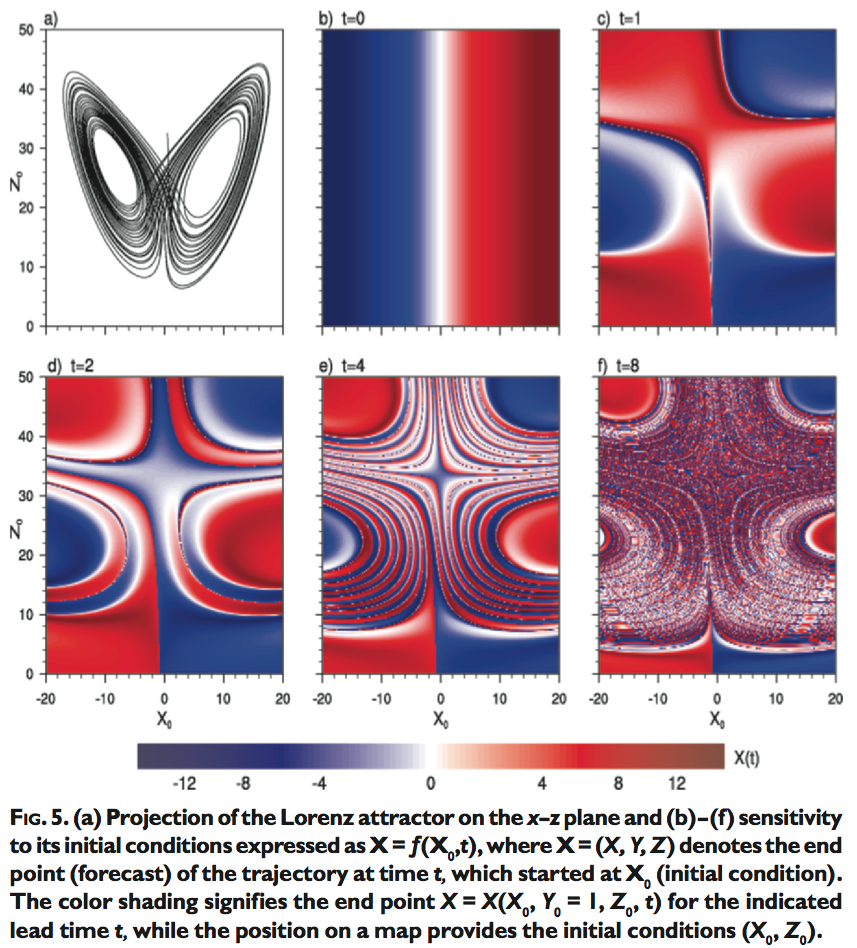
\includegraphics[height=33pc,width=33pc,angle=0]{figs/lorenz_attractor.png}
        \caption{\small Fig. 5 from \cite{hohenegger2007predictability}. (a) Projection of the Lorenz attractor on the $x$-$z$ plane and (b)–(f) sensitivity to its initial conditions expressed as $X = ƒ(X_0,t)$, where $X = (X, Y, Z)$ denotes the end point (forecast) of the trajectory at time $t$, which started at $X_0$ (initial condition). The color shading signifies the end point $X = X(X_0, Y_0 = 1, Z_0, t)$ for the indicated lead time t, while the position on a map provides the initial conditions $(X_0, Z_0)$.}
        \label{fig:lorenz}
    \end{center}
\end{figure}




% UTILIZING CONVECTIVE-SCALE ENSEMBLES
\chapter{Convective-Scale Ensembles}
\label{ensembles}
%!TEX root = generalexam.tex

% BEGIN CHAPTER

\cite{schwartz2010camresolution} demonstrated that quantitative precipitation forecasts benefit greatly from the use of high-resolution numerical models in both a deterministic and probabilistic framework. This is an important finding in that a majority of studies regarding cloud-resolving models used for producing forecast guidance more than a few hours in advance tend to be focused on deterministic results. It opens the door to such questions as, ``What should a storm-scale ensemble forecast system look like?'' It is becoming well established that convection-allowing models have shown improved skill in identifying regions where rare meteorological events associated with convection may occur -- especially when considered in the context of traditional numerical  models with parameterized convection. What has yet to be objectively demonstrated is how to best represent the uncertainty information from convection-allowing models.


Ensemble prediction systems have been a powerful tool in quantifying uncertainty in numerical forecasts; probabilistic forecast information is inherent in the ensemble generated output. For any given forecast field, one simply has to divide the number of numerical forecasts in which an event occurred divided by the number of numerical forecasts in which the event did not occur to receive a probability of an event occurring. One drawback to this method, however, is that probabilities generated are discrete, in intervals determined by the number of members in the ensemble. This poses significant challenges in how best to present traditional verification metrics such as reliability. One way to increase the resolution of the inherent probabilistic forecasts of ensemble prediction systems, one must increase the number of members, which, of course, requires additional computations resources or running numerical models at coarser grid spacing.


\cite{hamill1998eps} proposed a method for generating continuous probabilities from finite ensemble forecasts based on the ensemble's historical performance. This is best explained in an example. Consider a 4-member ensemble, where the sorted (highest-to-lowest) accumulated precipitation forecasts (in mm) are 40, 30, 20, and 10. To generate the probability that 25 mm or more of precipitation would accumulate, count the number of ensemble member's forecasts that exceed 25 mm and divide by the total number of ensemble members plus 1. Thus, $2 / (4+1) = 0.4$. However, that is the probability of exceeding 30 mm, no 25 mm; the probability of exceeding 25 mm should actually be greater than that of exceeding 30 mm. To account for this, determine the probability of exceeding the next lower ensemble threshold. Thus, $3 / (4+1) = 0.6$, yield a probability of exceedance of 60\%. The probability of exceeding 25 mm lies somewhere between 0.4 and 0.6. To determine the probability of exceeding 25 mm is determined by interpolating between the two values; the exact nature of this interpolation is determined by the ensemble's historical rank histogram.


The reason for using one more than the number of ensemble members in the divisor, instead of the number of ensemble members, becomes apparent when considering the two cases in which every ensemble member is either above or below the threshold at which one carries out the probability of exceedance. If every ensemble member produces precipitation, it is assumed that the probability of precipitation accumulating is unity. To put it another way, the probability of exceeding 0 mm is given a 100\% probability. If an ensemble member's forecast exceeds the forecast threshold (in the previous example it was 25 mm), the resulting (grid point) probability of exceedance is given by


$$
    POE = 1 - \left[\left(\frac{THRESH}{AMT_{min}}\right)(1 - PROB_{min})\right],
$$


\noindent where, $POE$ is the probability of exceeding the forecast threshold, given by $THRESH$, $AMT_{min}$ is the minimum forecast amount from any ensemble member (at the grid point), and $PROB_{min}$ is the probability of exceeding the amount forecast by the lowest ensemble member.


A similar exercise is undertaken for the case where every ensemble member forecasts amounts less than the threshold. In this case a linear extrapolation doesn't make sense. Considering again the example ensemble presented earlier, the probability of exceeding 50 mm should be greater than the probability of exceeding 100 mm. Thus, instead of a linear interpolation, a Gumbel distribution is used.


Unfortunately, as mentioned above, this method only makes use of forecasts at individual grid points. The very nature of a WoF paradigm is to produce forecasts of rare (in space and time) events. The intrinsic nature of rare events makes it unlikely that two separate high-resolution model forecasts would place identical phenomena at the same grid point, even for generally similar forecasts. Thus, creation and calibration of probabilistic forecasts of rare-events, such as those envisioned by WoF, requires a new approach.


This is a non-trivial task. Convection-allowing ensemble prediction systems are relatively new in the context of numerical modeling. Too little is known about the performance characteristics of convection-allowing models in explicitly predicting rare convective events, let alone understanding the performance of convection-allowing ensembles. This can be attributed to a number of reasons, chiefly among them is the relatively short duration of storm-scale ensemble forecast efforts \citep{done2004cams, clark2012overview} and poor observational datasets of rare convective hazards (e.g., \citealp{doswell1988stormreports, weiss2002stormreports, trapp2006stormreports, ortega2009shave}).


The composition of an ensemble's membership is an unsettled question in meteorological communities. Some believe that since initial condition errors tend to grow rapidly, that ensembles should consist solely of initial condition perturbations. Others argue that differences in model physics provide the most diversity of forecasts and thus ensembles should include some variations in physics packages. And still others argue that varying the model used produces the greatest impacts on at least features related to the land surface (surface temperature, moisture and winds -- all important in convective scale forecasts) is an important characteristic in an ensemble (\citealp{stensrud2000epscreation, eckel2005ensemble} and references contained within).  Ultimately, ensemble membership will most likely consist of combinations from all three viewpoints, but what remains to be seen what the optimal contributions from the various viewpoints will be.


There is a cost associated with adding a member to an ensemble. This cost is either computation, coming from either decreasing the horizontal and/or vertical grid spacing of every member, or monetary, stemming from the increased cost associated with additional computing and storage power. Thus a trade-off must be made when determining an ensemble's size. Arising out of this trade-off is the question, ``What is point of diminishing return with respect to ensemble size?'' In other words, at what point does the cost of adding additional members outweigh the contribution to forecast skill?


In some regards, these problems and questions have been the focus of an extraordinary collaborative effort between NSSL, SPC, and CAPS for several years through the Hazardous Weather Testbed Experimental Forecast Program (HWT-EFP). Although storm-scale models have been an important part of the HWT-EFP for a number of years, in 2011 CAPS was able to produce over 50, 4-km grid spacing numerical forecasts nightly. This has afforded HWT-EFP collaborators and participants an extraordinary opportunity to gain insights into how to create, transmit, visualize, and verify a storm-scale ensemble forecast system (SSEF). Additionally, this past year, Israel Jirak and Steve Weiss, both at SPC, championed the notion of a Storm-Scale Ensemble of Opportunity (SSEO) forecast system. The idea here was to take all the ``regularly'' available storm-scale forecasts and combine them together via post-processing techniques to produce probabilistic guidance of severe convective hazards.


What follows are thoughts on activities the HWT-EFP can undertake to examine these issues.




%%%%%%%%%%%%%%%%%%%%%%%%%%%%%
\section{Ensemble Membership}
%%%%%%%%%%%%%%%%%%%%%%%%%%%%%

The question of ensemble membership is difficult. The most obvious way to address this issue is to run various sets of ensembles and then examine the output. Fortunately, CAPS has been extremely successful in acquiring computational resources necessary to produce storm-scale ensemble forecasts. In 2010, CAPS produced a 15-member SSEF with grid spacing at 4 km, which grew to over 50 members in 2011. The 50 member SSEF of 2011 was comprised of several smaller ensembles including a 5 member ensemble, 15\footnote{The 15 member ensemble consisted of the same 15 members from 2010.} member ensemble, 18 member ensemble, and a 25\footnote{The 25th member was unavailable for a majority of the 2011 HWT-EFP.} member ensemble\footnote{The 5 member ensemble was a subset of the 15 member ensemble, which was a subset of the 25 member ensemble.} In the 25-member ensemble, 18 of the members were WRF-ARW cores, 5 were WRF-NMM (Nonhydrostatic Mesoscale Model) cores, and 1 was an Advanced Regional Prediction System (ARPS) Model. These models were initialized with a variations in initial and lateral boundary conditions and utilized different physics configurations. A list of the model configurations is given at the end of this chapter in Table \ref{ensemble_members}.


This unique dataset allows for simultaneous investigation into the questions previously presented.  The impacts of ensemble size can be explicitly evaluated from the perspective of 5, 15, and 25 members. The 18 member ensemble allowed for investigations into the impact of various choices for microphysics and planetary boundary layer (and combinations thereof), isolated from impacts of changing initial conditions. Granted a single HWT-EFP experiment, which consist of approximately 5 weeks of forecasts, is too small of a time-period (sample size) to draw vision altering results, however, it does allow one to frame the debate and develop questions for future investigations.




%%%%%%%%%%%%%%%%%%%%%
\section{Application}
%%%%%%%%%%%%%%%%%%%%%

The WoF vision of high-resolution, short-term forecasts of explicit severe convective hazards is still a long way from fruition on a CONUS scale, if for no other reason the National Oceanic and Atmospheric Administration's (NOAA) budget for both the National Weather Service and Office∫ of Ocean and Atmospheric Research does not allow for the necessary increases in computing power. In fact, the NWS National Centers for Environmental Prediction (NCEP) had to forgo its latest computing infrastructure upgrade and isn't scheduled for another one until 2014 (Weiss, personal communication 2011). However, much can be done in the interim.


Even though CONUS scale ensemble prediction systems capable of explicitly predicting convective hazards are many years off, convective scale ensembles, such as those run during the HWT-EFP, are certainly possible in the interim. One such real-time example of this is the High-Resolution Rapid Refresh (HRRR) model is now run hourly out to 15-hours \citep{smith2008hrrr}. Although a single deterministic model, research into the skill of time-lagged ensembles derived from models such as the HRRR should be evaluated. Along the same lines, a grass-roots type movement ensemble has been developed in-house at the SPC. At any given time there are approximately a half dozen or more storm-scale models that are valid. The ides behind the ``Storm-Scale Ensemble of Opportunity'' is that useful information can be gleaned from this ``opportunistic'' ensemble comprised of models provided by NSSL and NCEP's Environmental Modeling Center. Grass-roots approaches to furthering the WoF vision will continue to play a significant role over the next decade in answering the question of how to best apply storm-scale ensemble frameworks in operational settings.




%%%%%%%%%%%%%%%%%%%%%%
\section{Optimization}
%%%%%%%%%%%%%%%%%%%%%%

The question of ensemble optimization is rather open ended. What does it mean to optimize an ensemble anyways? Is determining ensemble membership part of the process of optimization? What about post-processing ensemble output? At least in the short term, the two are most likely related via the following question, ``What is the fewest number of members necessary to generate calibrated probabilistic forecasts when combined with statistical post-processing techniques?''  In a round about way, \cite{sobash2011kde} touched on this problem by utilizing kernel density estimation in a forecast sense. The method proposed by Sobash and coauthors took deterministic output and generated probabilistic fields. \cite{marsh2012callibration} expanded the kernel density estimation by developing a method to determine the the approximate smoothing values in an objective manner. Although this work was done in a deterministic framework, there are several methods in which it can be extended for using with ensembles. \cite{wilks2002smoothing} demonstrated that ensemble reliability can be improved by smoothing the output, which this method inherently does.


The benefit to approaches such as this will be computational savings by reducing the number of ensemble members necessary to capture the spread of possibilities and produce reliable forecasts. WoF will be computationally constrained for many years to come, so any method that can reduce the number of members necessary deserves further investigation.


Two drawbacks to statistical post processing techniques are the need for relatively large sample size of stable forecasts and high-resolution observations of the fields being forecast. The primary method to address the former problem is to simply wait long enough to create a sample of forecasts in which meaningful statistical techniques become appropriate. The latter method requires investment in methods of collecting high-resolution observations. Projects such as the Severe Hazards Analysis and Verification Experiment (SHAVE; \citealp{ortega2009shave}) and detailed surveys of high-impacts events, such as the damage surveys conducted of the 03 May 1999 tornado outbreak, are essential in establishing the observational datasets required for statistical post processing (not to mention, verification of forecasts).




%%%%%%%%%%%%%%%%%%%%%%%
\section{Visualization}
%%%%%%%%%%%%%%%%%%%%%%%

The issue of how to visualize information from high-resolution, storm-scale ensembles. Traditionally, forecasters are used to evaluating output from deterministic models. Forecasters can look, or at least give themselves the false sense of having looked, at everything there is to examine from a single model. As the WoF vision is realized, the flow of information will quickly make obsolete the option of examining all the model output. Instead methods of quickly visualizing \emph{and synthesizing} the output will be necessary. Recent HWT-EFPs have begun addressing this issue. Below is a sample of the work that has been started in this area, and it's potential benefits. It is a good start, but more work needs to be done.


\cite{marsh2010sls} utilized a web-display that allowed forecasters to choose various various smoothing parameters and view the resulting output from the 2010 HWT-EFP SSEF. Forecasters who preferred seeing detail in the probabilistic plots could choose smaller smoothing parameters and those who were comfortable with the larger smoothing parameters could choose those as well.  Additionally this web-display allowed forecasters to see the hourly probabilities of their choosing translate through space and time at hourly intervals, giving the forecaster a sense of how the ensemble as a whole evolved during that time frame.


In the 2011 HWT-EFP\footnote{Available at \url{http://hwt.nssl.noaa.gov/Spring_2011/ci_ens.php?date=20110524&p=6}.}, Marsh expanded the web-display to include many more options. Forecasters and researchers could choose to loop individual smoothed forecasts or the smoothed ensemble probabilities of various smoothing parameters. Since the ensemble was rather large, forecasters and researchers had an option to dynamically set the number of panels to display (typically in multiples of 3), and could choose what field to display in any of the windows. Additionally, forecasters and researchers could choose to turn on and off the option of displaying any of the individual members' forecasts of the phenomena in question. This allowed forecasters and researchers to visualize how phenomena from individual members contributed to the probabilities for that member. Additionally, forecasters and researchers to be able to overlay the specific phenomena from any member on the background probability of the ensemble. Feedback from participants suggests that web-displays of this sort are absolutely crucial for people evaluating ensembles to be able to interrogate the data while keeping a sense of the probabilistic information offered by the ensemble.


Additional displays are either in the works or need to be created. Marsh has committed to creating the capability display forecast soundings from ensembles in a manner that is convenient to compare them to observations from both traditional (radiosondes) and non-traditional sources (radiometers, Doppler LIDARs, etc) on time scales of the observing platforms. In other words, being able to display model soundings at 5 minute intervals in comparison to a radiometer. Tools like this should allow for researchers to quickly visualize and synthesize how a model predicted boundary layer is evolving compared to those observed.


Additional effort should be given toward means of extracting statistical information from individual members as well as the entire ensemble in a efficient and dynamical manner.




%%%%%%%%%%%%%%%%%%%%%%
\section{Verification}
%%%%%%%%%%%%%%%%%%%%%%

Any discussion about convective ensembles and the WoF initiative would be remiss if it didn't include discussion regarding verification. As numerical models continue to run at finer and finer grid spacing, it becomes harder and harder to measure improvements in the models' performances. Verification metrics ultimately depend on what it is one cares about. If someone cares about improving forecast skill, a different norm might be chosen than someone who cares about improving model dynamics \citep{hacker2005predictability}. Since WoF has an explicit goal related to prediction of high-impact convective hazards, this discussion will focus on the problem of improving forecast skill.


As briefly touched upon earlier in this chapter, a major component surrounding the issue of improving forecast skill is that as the number of grid points contained within a model increase, the number of grid points available for a model to resolve it's solution increases. Traditional verification metrics penalize high-resolution models for displacement errors, even if the high-resolution model conveyed the general idea of the forecast. For example, traditional verification metrics would tend to lead users in believing a model had very poor skill if the model was off on its forecast by one grid space everywhere, even though human forecasters would most likely consider it a successful forecast. As noted in \cite{clark2009comparison}, and discussed yearly among HWT-EFP collaborators, better verification metrics must be explored, and object-based metrics are a leading candidate.


Another problem regarding the measuring of forecast skill is that producing the most skillful forecasts (such as in terms of reliability) might not provide the most useful information to forecasters. Take for example the work by \cite{marsh2012calibration}. Marsh and coauthors have developed a method to generate probabilistic forecasts of rare events from deterministic forecasts that are more statistically reliable than the 2011 HWT-EFP 25 member SSEF (Figs. \ref{fig:nssl}, \ref{fig:ssef}, and \ref{fig:roc rely}). However subjective impressions of the resulting output is that the probability field is ``too smooth''. During the 2011 HWT-EFP most visiting forecasters did not use the product in the course of their forecast process.  Forecasters have a tendency to want to look at fields that do not smooth out the underlying signal and thus prefer looking at fields with less smoothing, even if it the resulting probabilistic fields are not reliable. Verification metrics that adequately capture the subconscious metrics used by human forecasters are sorely needed.


Lastly, as ensemble simulations, such as the HRRR and, in particular, those produced by CAPS, become more common, \cite{hamill2006trueskill} offer a warning of sorts regarding understanding model skill. Model skill must be understood in the context of the climatological event frequency, especially across vast spatial domains. Is a model's perceived skill the result of actual skill or spatially varying climatological frequencies? In particular, \cite{hamill2006trueskill} urge caution when using the Brier Skill Score, Relative Operating Characteristics, and Equitable Threat Scores. In particular, caution is implored when positive skill is diagnosed from reference climatological forecasts when distinct climatologies can be identified in subsets of the parent dataset. This perceived skill may actually be the result of underlying differences in the various distinct climatologies represented by a single climatological norm.


To address these potential issues, verification should be carried out over each of regions that have distinct climatologies. Alternatively, consider computing skill scores from each distinct climatology using local climatological distributions, such as exceeding various quantiles. This implicitly accounts for varying means and variances across the different climatologies and ensures that the same fraction of data are used. Ultimately, whatever metric is used, the specific details should be fully disclosed for reproducibility.




%%%%%%%%%%%%%%%%%%%%%%%%%%%
%!TEX root = prospectus.tex


% ENSEMBLE DATA



%%%%%%%%%%%%%%%%%%%%%%%%%%%%%%%%%%%%%%%%%%%%%%%%%
%%%                                           %%%
%%%                  TABLES                   %%%
%%%                                           %%%
%%%%%%%%%%%%%%%%%%%%%%%%%%%%%%%%%%%%%%%%%%%%%%%%%

\newpage

\begin{center}
    \renewcommand{\arraystretch}{3}
    \centering
    \singlespace
    \rowcolors{2}{gray!20}{white}
    \begin{longtable}{|c|c|c|c|c|c|c|}
        \caption[Configurations for the 2011 CAPS Ensemble Members]
        {Configurations for the 2010 and 2011 CAPS Ensemble Members. Members listed in red are those used in both 2010 and 2011.}
        \label{ensemble_members} \\

        % Header for the first page
        \hline
        \rowcolor{gray!60}
        \member{\textbf{Member}} &
        \ic{\textbf{Initial Conditions}} &
        \bc{\textbf{Boundary Conditions}} &
        \radar{\textbf{Radar Data}} &
        \microphysics{\textbf{Microphysics}} &
        \lsm{\textbf{LSM}} &
        \pbl{\textbf{PBL}} \\
        \hline
        \endfirsthead

        % Header for remaining pages
        \multicolumn{7}{c}{{\tablename} \thetable{} -- Continued} \\
        \hline
        \rowcolor{gray!60}
        \member{\textbf{Member}} &
        \ic{\textbf{Initial Conditions}} &
        \bc{\textbf{Boundary Conditions}} &
        \radar{\textbf{Radar Data}} &
        \microphysics{\textbf{Microphysics}} &
        \lsm{\textbf{LSM}} &
        \pbl{\textbf{PBL}} \\
        \hline
        \endhead

        %This is the footer for all pages except the last page of the table...
        \multicolumn{7}{l}{{Continued on Next Page \ldots}} \\
        \endfoot

        %This is the footer for the last page of the table...
        \hline \hline
        \multicolumn{7}{l}{Note 1: For all members, \emph{cu\_physics} = None} \\
        \multicolumn{7}{l}{Note 2: For all ARW members, \emph{ra\_lw\_physics} = RRTM} \\
        \multicolumn{7}{l}{Note 3: For all ARW members, \emph{ra\_sw\_physics} = Goddard} \\
        \multicolumn{7}{l}{Note 4: For nmm\_cn, nmm\_m2, \& nmm\_m3, \emph{ra\_lw\_physics} = GFDL;
            \emph{ra\_sw\_physics} = GFDL} \\
        \multicolumn{7}{l}{Note 5: For nmm\_m4 \& nmm\_m5, \emph{ra\_lw\_physics} = RRTM;
            \emph{ra\_sw\_physics} = Dudhia} \\
        \multicolumn{7}{l}{Note 6: The arps member uses Chou/Suarex for radiation.} \\
        \multicolumn{7}{l}{Note 7: Ferrier+ refers to a subset of changes in the updated
            version now in NEMS/NMMB.} \\

        \endlastfoot

        % Member 1 of 24
        \hline
        \coremem\member{arw\_cn} &
        \coremem\ic{00Z ARPS 3DVAR \& Cloud Analysis} &
        \coremem\bc{00Z NAM Forecast} &
        \coremem\radar{Yes} &
        \coremem\microphysics{Thompson} &
        \coremem\lsm{Noah} &
        \coremem\pbl{MYJ} \\

        % Member 2 of 24
        \hline
        \coremem\member{arw\_m4} &
        \coremem\ic{arw\_cn + em\_p1\_pert} &
        \coremem\bc{21Z SREF em\_p1} &
        \coremem\radar{Yes} &
        \coremem\microphysics{Morrison} &
        \coremem\lsm{RUC} &
        \coremem\pbl{YSU} \\

        % Member 3 of 24
        \hline
        \coremem\member{arw\_m5} &
        \coremem\ic{arw\_cn + em\_p2\_pert} &
        \coremem\bc{21Z SREF em\_p2} &
        \coremem\radar{Yes} &
        \coremem\microphysics{Thompson} &
        \coremem\lsm{Noah} &
        \coremem\pbl{QNSE} \\

        % Member 4 of 24
        \hline
        \coremem\member{arw\_m6} &
        \coremem\ic{arw\_cn - nmm\_p1\_pert} &
        \coremem\bc{21 SREF nmm\_p1} &
        \coremem\radar{Yes} &
        \coremem\microphysics{WSM6} &
        \coremem\lsm{RUC} &
        \coremem\pbl{QNSE} \\

        % Member 5 of 24
        \hline
        \coremem\member{arw\_m7} &
        \coremem\ic{arw\_cn + nmm\_p2\_pert} &
        \coremem\bc{21Z SREF nm\_p2} &
        \coremem\radar{Yes} &
        \coremem\microphysics{WDM6} &
        \coremem\lsm{Noah} &
        \coremem\pbl{MYNN} \\

        % Member 6 of 24
        \hline
        \coremem\member{arw\_m8} &
        \coremem\ic{arw\_cn + rsm\_n1\_pert} &
        \coremem\bc{21Z SREF rsm\_n1} &
        \coremem\radar{Yes} &
        \coremem\microphysics{Ferrier} &
        \coremem\lsm{RUC} &
        \coremem\pbl{YSU} \\

        % Member 7 of 24
        \hline
        \coremem\member{arw\_m9} &
        \coremem\ic{arw\_cn - etaKF\_n1\_pert} &
        \coremem\bc{21Z SREF etaKF\_n1} &
        \coremem\radar{Yes} &
        \coremem\microphysics{Ferrier} &
        \coremem\lsm{Noah} &
        \coremem\pbl{YSU} \\

        % Member 8 or 24
        \hline
        \coremem\member{arw\_m10} &
        \coremem\ic{arw\_cn + etaKF\_p1\_pert} &
        \coremem\bc{21Z SREF etaKF\_p1} &
        \coremem\radar{Yes} &
        \coremem\microphysics{WDM6} &
        \coremem\lsm{Noah} &
        \coremem\pbl{QNSE} \\

        % Member 9 of 24
        \hline
        \coremem\member{arw\_m11} &
        \coremem\ic{arw\_cn - etaBMJ\_p1\_pert} &
        \coremem\bc{21Z SREF etaBMJ\_p1 } &
        \coremem\radar{Yes} &
        \coremem\microphysics{WSM6} &
        \coremem\lsm{RUC} &
        \coremem\pbl{MYNN} \\

        % Member 10 of 24
        \hline
        \coremem\member{arw\_m12} &
        \coremem\ic{arw\_cn + etaBMJ\_p1\_pert} &
        \coremem\bc{21Z SREF etaBMJ\_p1} &
        \coremem\radar{Yes} &
        \coremem\microphysics{Thompson} &
        \coremem\lsm{RUC} &
        \coremem\pbl{MYNN} \\

        % Member 11 of 24
        \hline
        \member{arw\_m13} &
        \ic{arw\_cn + rsm\_p1\_pert} &
        \bc{21Z SREF rsm\_p1} &
        \radar{Yes} &
        \microphysics{M-Y} &
        \lsm{Noah} &
        \pbl{MYJ} \\

        % Member 12 of 24
        \hline
        \member{arw\_m14} &
        \ic{arw\_cn + em\_n1\_pert} &
        \bc{21 SREF em\_n1} &
        \radar{Yes} &
        \microphysics{Ferrier+} &
        \lsm{Noah} &
        \pbl{YSU} \\

        % Member 13 of 24
        \hline
        \member{arw\_m15} &
        \ic{arw\_cn + em\_n2\_pert} &
        \bc{21Z SREF em\_n2} &
        \radar{Yes} &
        \microphysics{WSM6} &
        \lsm{Noah} &
        \pbl{MYNN} \\

        % Member 14 of 24
        \hline
        \member{arw\_m16} &
        \ic{arw\_cn + nmm\_n1\_pert} &
        \bc{21Z SREF nmm\_n1} &
        \radar{Yes} &
        \microphysics{Ferrier+} &
        \lsm{Noah} &
        \pbl{QNSE} \\

        % Member 15 of 24
        \hline
        \member{arw\_m17} &
        \ic{arw\_cn + nmm\_n2\_pert} &
        \bc{21Z SREF nmm\_n2} &
        \radar{Yes} &
        \microphysics{Thompson} &
        \lsm{Noah} &
        \pbl{ACM2} \\

        % Member 16 or 24
        \hline
        \member{arw\_m18} &
        \ic{arw\_cn + rsm\_p2\_pert} &
        \bc{21Z SREF rsm\_p2} &
        \radar{Yes} &
        \microphysics{WSM6} &
        \lsm{Noah} &
        \pbl{MYJ} \\

        % Member 17 of 24
        \hline
        \member{arw\_m19} &
        \ic{arw\_cn + rsm\_n1\_pert} &
        \bc{21Z SREF rsm\_n1} &
        \radar{Yes} &
        \microphysics{M-Y} &
        \lsm{Noah} &
        \pbl{MYJ} \\

        % Member 18 of 24
        \hline
        \member{arw\_m20} &
        \ic{arw\_cn + rsm\_n2\_pert} &
        \bc{21Z SREF rsm\_n2} &
        \radar{Yes} &
        \microphysics{M-Y} &
        \lsm{RUC} &
        \pbl{ACM2} \\

        % Member 19 of 24
        \hline
        \coremem\member{nmm\_cn} &
        \coremem\ic{00Z ARPS 3DVAR \& Cloud Analysis} &
        \coremem\bc{00Z NAM Forecast} &
        \coremem\radar{Yes} &
        \coremem\microphysics{Ferrier} &
        \coremem\lsm{Noah} &
        \coremem\pbl{MYJ} \\

        % Member 20 of 24
        \hline
        \member{nmm\_m2} &
        \ic{nmm\_cn + em\_n2\_pert} &
        \bc{21 SREF em\_n2} &
        \radar{Yes} &
        \microphysics{Ferrier+} &
        \lsm{Noah} &
        \pbl{MYJ} \\

        % Member 21 of 24
        \hline
        \coremem\member{nmm\_m3} &
        \coremem\ic{nmm\_cn + nmm\_n1\_pert} &
        \coremem\bc{21Z SREF nmm\_n1} &
        \coremem\radar{Yes} &
        \coremem\microphysics{Thompson} &
        \coremem\lsm{Noah} &
        \coremem\pbl{MYJ} \\

        % Member 22 of 24
        \hline
        \coremem\member{nmm\_m4} &
        \coremem\ic{arw\_cn + nmm\_n2\_pert} &
        \coremem\bc{21Z SREF nmm\_n2} &
        \coremem\radar{Yes} &
        \coremem\microphysics{WSM6} &
        \coremem\lsm{RUC} &
        \coremem\pbl{MYJ} \\

        % Member 23 of 24
        \hline
        \coremem\member{nmm\_m5} &
        \coremem\ic{arw\_cn + em\_n1\_pert} &
        \coremem\bc{21Z SREF em\_n1} &
        \coremem\radar{Yes} &
        \coremem\microphysics{Ferrier} &
        \coremem\lsm{RUC} &
        \coremem\pbl{MYJ} \\

        % Member 24 or 24
        \hline
        \coremem\member{arps\_cn} &
        \coremem\ic{00Z ARPS 3DVAR \& Cloud Analysis} &
        \coremem\bc{00Z NAM Forecast} &
        \coremem\radar{Yes} &
        \coremem\microphysics{Lin} &
        \coremem\lsm{Force Restore} &
        \coremem\pbl{??? ???} \\
        \hline

    \end{longtable}
\end{center}




\label{2011ssef}
%%%%%%%%%%%%%%%%%%%%%%%%%%%




%%%%%%%%%%%%%%%%%%%%%%%%%%%%%%%%%%%%%%%%%%%%%%%%%
%%%%%%%%%%           FIGURES           %%%%%%%%%%
%%%%%%%%%%%%%%%%%%%%%%%%%%%%%%%%%%%%%%%%%%%%%%%%%

\newpage


\begin{figure}
    \begin{center}
        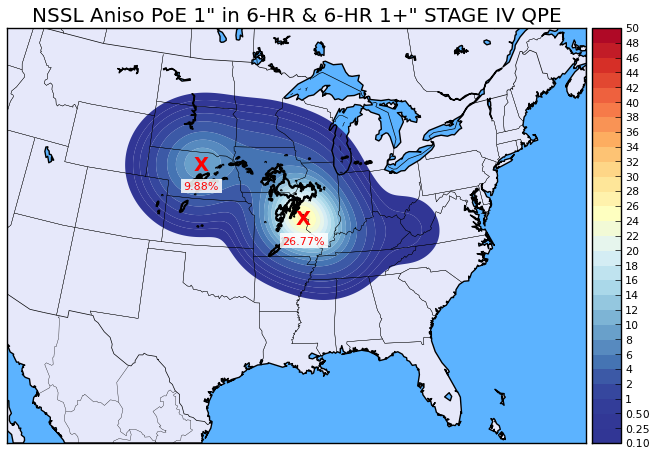
\includegraphics[scale=0.50]{figs/nssl.png}
        \caption{\small Sample probabilistic post-processed output generated from the NSSLWRF using the method put forth by \cite{marsh2012calibration}. The forecast threshold is 25.4 mm in 6 h.}
        \label{fig:nssl}
    \end{center}
\end{figure}


\begin{figure}
    \begin{center}
        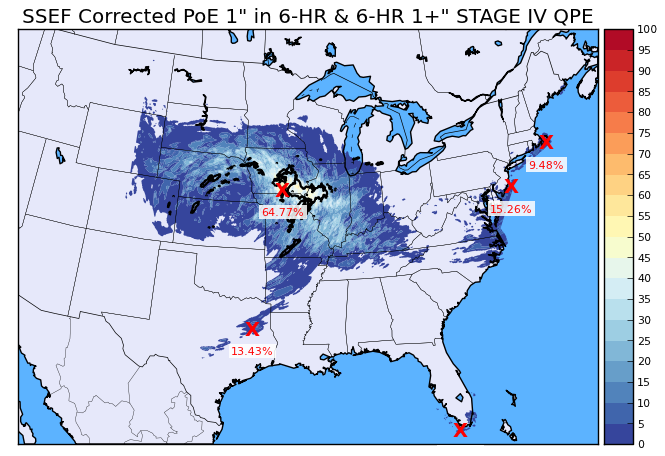
\includegraphics[scale=0.50]{figs/ssef.png}
        \caption{\small Sample probabilistic post-processed output created from the HWT-EFP 2011 25 member storm-scale ensemble forecast system. The probabilisties here were generated using the method put forth by \cite{hamill1998eps}. The forecast threshold is 25.4 mm in 6 h, and is valid for the same time period as in Fig. \ref{fig:nssl}.}
        \label{fig:ssef}
    \end{center}
\end{figure}


\begin{figure}
    \begin{center}
        \includegraphics[scale=0.4]{figs/roc_rely.pdf}
        \caption{\small The ROC curve and reliability diagram comparing probabilistic output from the NSSLWRF using the methods of \cite{marsh2012calibration} as compared to the output generated from the 2011 HWT-EFP 25 member SSEF. Forecasts were only evaluated over time periods where both the SSEF and NSSLWRF were available.}
        \label{fig:roc rely}
    \end{center}
\end{figure}


% DISCUSSION
\chapter{Discussion}
\label{discussion}
%!TEX root = generalexam.tex

% BEGIN CHAPTER

Achieving WoF will be hard. Very hard. It \emph{is} hard. It will not happen overnight, but then again most things that are worth anything are worth working hard toward and waiting for.  No one individual will have all the answers and WoF will require a significant amount of collaboration amongst the many players.


This document presents some information regarding challenge facing WoF, but it only begins to scratch the surface.The American economy is still in the doldrums and Government is wanting to slash science funding.  Decreasing budgets for science, and in turn observing networks, will make establishing observational networks to aid a WoF system harder to afford.  Can a WoF system provide near continuous updates of high-resolution, calibrated, probabilistic information without having near continuous updates of high-resolution observations? If these observations are not going to be available, then add yet another hurdle WoF will need to overcome.


Questions also remain as to how forecasters will utilize probabilistic information in an operational setting.  The sheer amount of information that forecasters will be required to synthesize is unfathomable at this time.  The author remembers participating in an HWT-Experimental Warning Program (EWP) experiment investigating Phased Array Radar output. After examining what felt like hours worth of data, participants were informed they only has examined 20-30 minutes worth. Imagine a warning operations setting in which Phased Array Radar output with O(1 min) updates are being thrust upon a forecaster, combined with near real-time analyses from a multitude of ensembles.


WoF will require a significant upgrade to infrastructure and bandwidth. As is stands now, personal communication with operational forecasters in local weather service offices complain that the bandwidth is not sufficient to acquire all of the information available now.  What happens when a WoF system, and the (hopefully) high-resolution observations that come with WoF, increases the amount of information by 10 fold or more?


Also, WoF would be remiss if it did not at least begin to think about how to convey this new, probabilistic information to a public who has an attention span with weather that waxes and wanes depending on the type of year.  How will people take to receiving probabilistic information in the context of severe convective hazards? Granted, probabilistic information will allow for individuals to compute personal cost/loss rations and determine for themselves what their personal thresholds of certainty need to be, but who is going to teach them to use WoF information in this manner? Meteorologists of the future will have to educate and communicate this information to a wide ranging of audiences ranging from the public at-large to emergency managers, to highly educated users (aka, other meteorologists). Future meteorologists will need to understand and be ready to trouble shoot data issued with a WoF system, in addition to actually knowing meteorology.  Meteorologists of the future will need to be a teacher, communicator, statistician, computer scientist, and meteorologist, all-in-one. Current academic curricula are not necessarily conducive to this, and making changes to curricula is no small task.


With all of what has been written here -- the discussion of the potential challenges and pitfalls -- the author is excited about the future of convective scale meteorology. Even if WoF is unobtainable in the near future, the number of advancements that will emanate from this initiative is northing short of a scientific revolution. It is an exciting time to be a convective scale meteorologist.


% REFERENCES
\references{ametsoc}{./bibliography/generalexam}


%%%%%%%%%%%%%%%%%%%%%%%%%%%%%%%%%%%%%%%%%%%%%%%%%%%%%%%%%%%%%%%%%%%%%
% END OF TEMPLATE
%%%%%%%%%%%%%%%%%%%%%%%%%%%%%%%%%%%%%%%%%%%%%%%%%%%%%%%%%%%%%%%%%%%%%
\end{document}